\documentclass[11pt,letterpaper]{article}

%% ─── Packages ───────────────────────────────────────────────────────────────
\usepackage[T1]{fontenc}
\usepackage[utf8]{inputenc}
\usepackage{geometry}
\usepackage{setspace}
\usepackage{amsmath,amssymb,amsthm}
\usepackage{mathtools}
\usepackage{booktabs}
\usepackage{array}
\usepackage{tabularx}
\usepackage{longtable}
\usepackage{multirow}
\usepackage{xcolor}
\usepackage{enumitem}
\usepackage{fancyhdr}
\usepackage{titlesec}
\usepackage{parskip}
\usepackage{graphicx}
\usepackage{tikz}
\usetikzlibrary{positioning,arrows.meta,shapes.geometric}
\usepackage{pgfplots}
\pgfplotsset{compat=1.18}
\usepackage{tcolorbox}
\tcbuselibrary{skins,breakable}
\usepackage{hyperref}
\usepackage{xurl}
\usepackage{bookmark}
\usepackage{cleveref}
\usepackage{caption}
\usepackage{subcaption}
\usepackage{mdframed}

%% ─── Geometry ───────────────────────────────────────────────────────────────
\geometry{
  letterpaper,
  top=1.0in, bottom=1.0in,
  left=1.15in, right=1.15in,
  headheight=14pt,
  headsep=18pt
}

%% ─── Color palette ──────────────────────────────────────────────────────────
\definecolor{SCblue}{RGB}{10,50,110}
\definecolor{SCaccent}{RGB}{0,110,170}
\definecolor{SCgold}{RGB}{170,120,0}
\definecolor{SCgray}{RGB}{75,85,95}
\definecolor{SClight}{RGB}{234,240,248}
\definecolor{SCgreen}{RGB}{15,95,55}
\definecolor{SCredrule}{RGB}{140,30,30}

%% ─── Hyperref ───────────────────────────────────────────────────────────────
\hypersetup{
  colorlinks=true,
  linkcolor=SCaccent,
  urlcolor=SCaccent,
  citecolor=SCgray,
  pdftitle={DSFB Structural Semiotics Engine for Semiconductor Process Control},
  pdfauthor={Riaan de Beer},
  pdfkeywords={semiconductor process control, fault detection, structural semiotics,
    DSFB, SECOM, admissibility envelope, deterministic diagnostics,
    augmentation layer, SPC, APC, run-to-run control}
}

%% ─── Typography ─────────────────────────────────────────────────────────────
\setstretch{1.09}
\emergencystretch=2em

%% ─── Section formatting ─────────────────────────────────────────────────────
\titleformat{\section}
  {\color{SCblue}\large\bfseries}
  {\thesection.}{0.6em}{}
  [\vspace{-4pt}\color{SCblue}\rule{\linewidth}{0.7pt}\vspace{2pt}]

\titleformat{\subsection}
  {\color{SCgray}\normalsize\bfseries}
  {\thesubsection}{0.5em}{}

\titleformat{\subsubsection}
  {\color{SCaccent}\normalsize\itshape}
  {}{0em}{}

\titlespacing{\section}{0pt}{14pt}{6pt}
\titlespacing{\subsection}{0pt}{10pt}{4pt}

%% ─── Header / Footer ────────────────────────────────────────────────────────
\setlength{\headheight}{22pt}
\pagestyle{fancy}
\fancyhf{}
\fancyhead[L]{\footnotesize\color{SCgray}\textit{DSFB Structural Semiotics Engine
  for Semiconductor Process Control}}
\fancyhead[R]{\footnotesize\color{SCgray}Invariant Forge LLC}
\fancyfoot[C]{\footnotesize\color{SCgray}\thepage}
\renewcommand{\headrulewidth}{0.4pt}
\renewcommand{\headrule}{\hbox to\headwidth{%
  \color{SCaccent}\leaders\hrule height \headrulewidth\hfill}}

%% ─── Theorem environments ───────────────────────────────────────────────────
\newtheoremstyle{scresult}
  {8pt}{6pt}{\itshape}{0pt}{\color{SCblue}\bfseries}{.}{0.5em}{}
\theoremstyle{scresult}
\newtheorem{theorem}{Theorem}
\newtheorem{corollary}[theorem]{Corollary}
\newtheorem{proposition}[theorem]{Proposition}
\newtheorem{definition}{Definition}
\newtheorem{remark}{Remark}

%% ─── Box environments ───────────────────────────────────────────────────────
\tcbset{
  lawbox/.style={
    enhanced, breakable,
    colback=white, colframe=SCblue,
    boxrule=1pt, arc=2pt,
    left=10pt, right=10pt, top=8pt, bottom=8pt,
    coltitle=black, colbacktitle=white,
    fonttitle=\bfseries,
    toptitle=2mm, bottomtitle=2mm
  },
  claimbox/.style={
    enhanced,
    colback=SClight, colframe=SCaccent,
    boxrule=0.8pt, arc=2pt,
    left=8pt, right=8pt, top=5pt, bottom=5pt
  },
  augbox/.style={
    enhanced,
    colback=white, colframe=SCgreen,
    boxrule=1pt, arc=2pt,
    left=8pt, right=8pt, top=5pt, bottom=5pt,
    borderline west={3pt}{0pt}{SCgreen}
  },
  warnbox/.style={
    enhanced,
    colback=white, colframe=SCgold,
    boxrule=0.8pt, arc=2pt,
    left=8pt, right=8pt, top=5pt, bottom=5pt,
    borderline west={3pt}{0pt}{SCgold}
  }
}

%% ─── List styling ────────────────────────────────────────────────────────────
\setlist[itemize]{
  leftmargin=1.4em, itemsep=2pt, parsep=0pt, topsep=4pt,
  label={\color{SCaccent}\small$\blacktriangleright$}
}
\setlist[enumerate]{
  leftmargin=1.6em, itemsep=2pt, parsep=0pt, topsep=4pt
}

%% ─── Math macros ─────────────────────────────────────────────────────────────
\newcommand{\R}{\mathbb{R}}
\newcommand{\norm}[1]{\left\|#1\right\|}
\newcommand{\Engine}{\mathcal{M}}
\newcommand{\envelope}{\mathcal{E}}
\newcommand{\bank}{\mathcal{H}}

%% ─── Caption styling ─────────────────────────────────────────────────────────
\captionsetup{
  font={small,color=SCgray},
  labelfont={bf,color=SCblue},
  skip=4pt
}

%% ═══════════════════════════════════════════════════════════════════════════
\begin{document}
%% ═══════════════════════════════════════════════════════════════════════════

%% ─── Title ───────────────────────────────────────────────────────────────────
\begin{center}
{\color{SCblue}\rule{\linewidth}{1.5pt}}
\vspace{8pt}

{\LARGE\bfseries\color{SCblue}
DSFB Structural Semiotics Engine\\[6pt]
for Semiconductor Process Control}

\vspace{6pt}
{\large\itshape\color{SCaccent}
A Deterministic Augmentation Layer for Typed Residual Interpretation\\
for Fault Detection and Run-to-Run Variation\\
in Advanced Manufacturing}

\vspace{8pt}
{\color{SCblue}\rule{\linewidth}{0.8pt}}

\vspace{12pt}

{\normalsize
Riaan de Beer\\
\texttt{riaan@invariantforge.net}\\
Chief Research Advisor, Invariant Forge LLC\\
ORCID: 0009-0006-1155-027X\\[4pt]
DOI: \textit{pending}\\
\texttt{https://github.com/infinityabundance/dsfb}\\[4pt]
Version 1.0 \quad March 2026
}

\vspace{12pt}

\begin{minipage}{0.88\linewidth}
\begin{center}
\textbf{Abstract}
\end{center}
\small
DSFB does not compete with SPC, EWMA, or FDC --- it augments them. Those
systems continue to operate unchanged. DSFB reads the residual streams they
already produce and returns a typed, deterministic, human-readable
interpretation of what the residuals mean structurally. On the SECOM public
benchmark under a fixed Stage~III read-only protocol, this augmentation
collapses 28{,}607 raw boundary episodes into 71 policy-governed
Review/Escalate episodes while preserving 104/104 labeled failure events.
Episode precision rises from a raw-boundary proxy of 0.36\% to 80.3\% ---
a 220$\times$ improvement in operator relevance. The upstream SPC and EWMA
systems are not modified, replaced, or disabled. If DSFB is removed, upstream
behavior is unchanged.

Semiconductor process monitoring already produces dense residual streams through
statistical process control (SPC), run-to-run and advanced process control
(APC), and fault detection and classification (FDC) systems, but operational
action is still dominated by scalar alarms that suppress temporal structure.
This paper studies the DSFB Structural Semiotics Engine as a deterministic
augmentation layer over those existing residual streams. It does not propose a
replacement controller or a new fab-wide monitoring stack. Instead, it maps
residual trajectories into explicit objects --- residual sign, admissibility
envelope, grammar state, and provenance-aware motif entries --- so that slow
drift, boundary approach, and structural excursion can be represented in a
typed and inspectable form.

The paper makes a bounded claim. It shows how deterministic intermediate
representations can support auditability arguments and operator review, and how
the DSFB formal objects can be instantiated using semiconductor observables such
as innovation residuals, control limits, and specification windows. It does not
prove SEMI standards compliance, completed qualification, universal superiority
over SPC/EWMA/FDC/ML baselines, or physical chamber-mechanism attribution from
public data alone.

The empirical evidence is Stage~III public-data evidence on the SECOM
dataset and its current Rust companion implementation. Under the fixed
operator-facing protocol, DSFB is evaluated strictly as a read-only downstream
layer over residuals already produced by existing SPC/EWMA/FDC-style
monitoring. In the selected SECOM configuration, the policy-governed DSFB
layer preserves 104/104 labeled failure events while reducing
investigation-worthy Review/Escalate decisions from 10{,}554 to 3{,}854
(63.5\%) and collapsing raw boundary episodes from 28{,}607 to 71
(99.75\%). Episode precision rises from a raw-boundary precision proxy of
0.36\% to 80.3\% (220.8x). The bounded empirical claim is therefore
operator-facing: DSFB does not alter upstream control logic, thresholds, or
actuation, but it converts a large residual review surface into a small set of
structured, human-readable episodes.

\vspace{4pt}
\begin{center}
\small
\textbf{Table A: Review Surface Reduction Efficiency (SECOM, Fixed Protocol)}\\[4pt]
\begin{tabular}{lrrr}
\toprule
\textbf{Stage} & \textbf{Count} & \textbf{Failure Recall} & \textbf{Episode Precision}\\
\midrule
Raw SPC boundary alarms & 28{,}607 & 100\% & 0.36\%\\
DSFB grammar episodes (Review/Escalate) & 71 & 100\% (104/104) & 80.3\%\\
\midrule
\textbf{Reduction factor} & \textbf{403$\times$} & \textbf{held} & \textbf{220.8$\times$ gain}\\
\bottomrule
\end{tabular}
\end{center}
\vspace{2pt}
\noindent\textit{DSFB does not change how the tool behaves; it changes how the engineer understands why the tool is behaving.}
\end{minipage}

\vspace{8pt}
{\color{SCblue}\rule{\linewidth}{0.8pt}}
\end{center}

\vspace{6pt}
{\footnotesize\color{SCgray}
\textbf{IP Notice.}
The theoretical framework, formal constructions, and supervisory methods described
herein constitute proprietary Background IP of Invariant Forge LLC
(Delaware LLC No.\ 10529072), with prior art established by this publication and
earlier Zenodo DOI publications by the same author. Commercial deployment requires
a separate written license. Reference implementations are released under
Apache~2.0. Licensing: \texttt{licensing@invariantforge.net}
}

\clearpage
\thispagestyle{plain}
\begingroup
\small
\setlength{\parindent}{0pt}
\setlist[itemize]{leftmargin=1.2em,itemsep=1pt,topsep=2pt}

\begin{center}
{\Large\bfseries DSFB: Non-Intrusive Structural Interpretation Layer for Semiconductor Monitoring Systems}
\end{center}

\textbf{1. WHAT IT DOES}
\begin{itemize}
  \item Converts residual alarm streams into structured episodes
  \item Reduces operator review surface by 99.75\%
  \item Raises event relevance from 0.36\% to 80.3\%
\end{itemize}

\textbf{2. WHAT IT DOES NOT DO}
\begin{itemize}
  \item Does not modify SPC/EWMA/FDC systems
  \item Does not change thresholds or control loops
  \item Does not introduce feedback into the process
\end{itemize}

\textbf{3. OPERATOR DELTA}
\begin{itemize}
  \item 28{,}607 $\rightarrow$ 71 review events ($-$99.75\%)
  \item 0.36\% $\rightarrow$ 80.3\% precision (220.8x)
  \item 63.5\% reduction in investigation load
  \item 104 / 104 failures preserved
\end{itemize}

\textbf{4. WHY THIS IS LOW RISK}
\begin{itemize}
  \item read-only
  \item side-channel execution
  \item deterministic outputs
  \item removable with zero system impact
\end{itemize}

\textbf{5. PHASE I DELIVERABLE}
\begin{itemize}
  \item integrate with real FDC streams
  \item validate on tool-level data
  \item measure operator burden reduction
\end{itemize}

\textbf{6. WHAT SUCCESS LOOKS LIKE}
\begin{itemize}
  \item fewer alarms
  \item higher signal relevance
  \item unchanged upstream systems
\end{itemize}

\vfill
\footnotesize
Evidence basis: selected SECOM operator row emitted by
\texttt{dsa\_operator\_delta\_targets.json} and
\texttt{episode\_precision\_metrics.json}.
\par
\endgroup


\clearpage
\tableofcontents
\clearpage

%% ═══════════════════════════════════════════════════════════════════════════
\section{Introduction}
\label{sec:intro}
%% ═══════════════════════════════════════════════════════════════════════════

\subsection{Motivation}

Semiconductor fabrication is among the most instrumented industrial processes
in existence. A modern 300mm fab produces millions of sensor measurements per
wafer run, spanning plasma power, gas flow rates, chamber pressure, optical
emission spectra, etch depth, deposition uniformity, and dozens of electrical
test parameters. Despite this instrumentation density, a central challenge
persists: distinguishing \emph{structured degradation} from \emph{normal
process variation} early enough to intervene before yield loss.

The dominant paradigm for residual-based process monitoring in semiconductor
manufacturing is statistical. Statistical Process Control (SPC) compares
measurements against control limits derived from historical variance. EWMA
controllers smooth innovation sequences into scalar signals that drive
run-to-run adjustments. Fault Detection and Classification (FDC) systems alarm
when multivariate sensor profiles deviate from empirical baselines. Probabilistic
fault detectors apply likelihood ratio tests or principal component analysis
to identify out-of-control conditions.

These methods share a structural limitation. They treat residuals primarily as
magnitudes to be compared against thresholds. A residual that grows slowly,
persistently, and directionally --- the signature of tool aging, chamber
seasoning drift, consumable degradation, or recipe creep --- may remain below
alarm thresholds for many wafer runs while its structural organization already
encodes the onset of a systematic process shift. By the time the shift becomes
statistically significant, the drift has been underway for hours or days.

\subsection{The Structural Opportunity}

The DSFB Structural Semiotics Engine addresses this limitation by treating
residual trajectories as primary inferential objects rather than sequences of
scalar discrepancies. The key insight is not new in spirit --- process engineers
already read drift patterns informally from SPC charts --- but it has not
previously been formalized into a deterministic and reusable
interpretive architecture.

The core claim of this paper is precise:

\begin{tcolorbox}[claimbox]
The innovation residuals produced by EWMA controllers, SPC systems, and
probabilistic fault detectors contain structured temporal information --- drift
direction, curvature of change, and admissibility relative to process
constraints --- that scalar alarm methods discard. The DSFB Structural Semiotics
Engine recovers and formalizes this structure as a typed, composable,
reusable interpretive layer.
\end{tcolorbox}

This is an augmentation claim, not a replacement claim. The engine does not
ask fabs to remove their SPC infrastructure, retrain their FDC models, or
replace their APC controllers. It reads the residuals those systems already
produce and provides a companion structural interpretation alongside them.

\subsection{Operational Objects and Decision Boundary}

The formal objects required for this paper are intentionally limited. The
residual $r(k)$ denotes the run-indexed deviation between a measured sensor or
derived process variable and its nominal reference. The admissibility envelope
$\mathcal{E}(k)$ defines the region considered operationally acceptable under
the chosen process limits or healthy-window statistics. The grammar layer maps
the residual trajectory to interpretable states such as \texttt{Admissible},
\texttt{Boundary}, and \texttt{Violation}. The heuristics bank records named
motifs together with provenance tags describing where those motifs came from.

These objects justify bounded decisions: continue monitoring, request
maintenance review, escalate an out-of-control event, or register a motif for
future interpretation. They do \emph{not} by themselves justify physical
root-cause attribution, autonomous recipe modification, cross-tool transfer
without recalibration, or standards-compliance claims.

\subsection{Relation to the DSFB Framework}

This paper is a domain application of the DSFB Structural Semiotics Engine
for General Systems~\cite{dsfb-semiotics-general}, which establishes the
foundational theory, formal results, and reference implementation. The full
theoretical treatment --- including the general definitions, theorems, and
proof-oriented discussion --- is contained in that
paper. The present paper is written to stand on its own for the semiconductor
reader: it restates only the formal objects and interpretations needed for
process control, then evaluates the bounded claim on the SECOM public dataset.

\subsection{Dual-Use Applicability}

\textbf{Dual-use applicability.}
The observer-only integration contract and deterministic audit trail described
in this paper are not specific to semiconductor manufacturing. Any domain in which
residual-producing controllers already exist --- aerospace component
manufacturing, defense electronics production, pharmaceutical process control,
automotive powertrain testing --- can receive the same augmentation layer without
modification to the primary control system. The same DSFB engine evaluated here
over SECOM residuals is deployable over FDC residuals in ITAR-controlled
manufacturing lines or AS9100-audited aerospace processes. This broad
applicability is a direct consequence of the non-intrusive architecture: the
engine reads residuals; it does not care what produced them.

\subsection{Scope, Assumptions, and Non-Claims}

The framework is deterministic in construction but does not claim that
semiconductor processes are noise-free or fully deterministic in ontology.
The claim is methodological: a deterministic interpretive layer can be built
over process residual trajectories even in settings where measurement noise,
lot-to-lot variation, and model imperfection remain present.

This paper does not claim:
\begin{itemize}
  \item that the semiotic approach subsumes SPC, EWMA, FDC, or probabilistic
        fault detection in all process regimes;
  \item that the fixed-protocol SECOM read-only demonstration (Stage~III) constitutes a complete empirical
        validation of the framework for all semiconductor process classes;
  \item that the current SECOM evidence supports chamber-mechanism attribution
        or physical root-cause identification;
  \item that admissibility envelopes derived from process specification windows
        are universally optimal or automatically calibrated;
  \item that the present manuscript establishes SEMI~E10 or E116 compliance,
        completed qualification, or deployment readiness;
  \item or that the heuristics bank, in its current form, exhausts the
        interpretive possibilities of real fab environments.
\end{itemize}

These limitations are addressed explicitly in Section~\ref{sec:limitations}.

\subsection{Contributions of This Paper}

\begin{enumerate}
  \item \textbf{Process control instantiation.} Formal mapping of DSFB
        objects --- residual signs, drift, slew, admissibility envelopes,
        grammar, and heuristics bank --- onto semiconductor process control
        constructs: innovation sequences, control limits, spec windows,
        operator review states, and residual motifs.

  \item \textbf{Augmentation architecture.} A formal characterization of
        how the structural semiotics engine sits on top of existing APC
        infrastructure without modifying it, and what the combination
        provides that neither component alone delivers.

  \item \textbf{Formal results in process context.} Direct interpretation
        of Law~1 (Structural Detectability Principle), Theorem~1
        (finite-time envelope exit), Theorem~9 (deterministic
        interpretability), and Theorem~10 (auditable early-warning
        inference) in the semiconductor process control setting.

  \item \textbf{SECOM operator-facing evaluation.} Application of the engine
        to the SECOM public dataset with explicit nominal model, envelope
        parameterization, bounded scalar comparators, typed motif outputs on
        real semiconductor data, and explicit review-surface / relevance /
        workload / recall reporting under a fixed protocol.

  \item \textbf{Runnable empirical companion.} A repo-local Rust crate and
        Colab notebook wiring that implement the fixed SECOM protocol, emit
        timestamped reports and bundles, provide a bounded SECOM calibration
        workflow, and expose the current PHM~2018 support boundary without
        claiming end-to-end PHM~2018 execution.

  \item \textbf{Qualification relevance.} A bounded argument for why
        deterministic and reproducible intermediate representations are
        relevant to later qualification workflows, without claiming that
        qualification is already complete.
\end{enumerate}

\subsection{Paper Map}

Section~\ref{sec:background} reviews semiconductor process control and its
residual monitoring infrastructure. Section~\ref{sec:related-work} surveys
related work in R2R control, FDC, SECOM benchmarking, and structural monitoring.
Section~\ref{sec:instantiation} formally
instantiates DSFB objects in the process control setting.
Section~\ref{sec:formal} interprets the key formal results in this domain.
Section~\ref{sec:nonintrusive} states the non-intrusive integration contract.
Section~\ref{sec:augmentation} develops the augmentation architecture.
Section~\ref{sec:incumbent} compares the framework against incumbent methods.
Section~\ref{sec:operator-value} states the operator-facing value proposition.
Section~\ref{sec:demonstration} presents the SECOM read-only evaluation.
Section~\ref{sec:failure-modes} states the operator-visible failure modes.
Section~\ref{sec:certification} discusses qualification relevance and the
integration pathway. Section~\ref{sec:limitations} states limitations.
Section~\ref{sec:conclusion} concludes.

%% ═══════════════════════════════════════════════════════════════════════════
\section{Non-Intrusive Integration}
\label{sec:nonintrusive}
%% ═══════════════════════════════════════════════════════════════════════════

This positioning is the load-bearing architectural claim of the paper. A fab
does not need to evaluate DSFB as a replacement for its monitoring
infrastructure. It evaluates DSFB as a zero-risk read-only companion that
makes its existing monitoring infrastructure more legible. The risk profile is
categorically different from deploying a new detector.

DSFB is positioned as a non-intrusive, observer-only layer. Existing
SPC/EWMA/FDC/APC systems remain authoritative. DSFB reads residuals and alarm
side taps, structures them into episodes, and emits advisory outputs only.

\begin{itemize}
  \item DSFB does not replace SPC, EWMA, APC, or FDC logic.
  \item DSFB does not write thresholds, controller gains, recipe values, or
        actuation commands.
  \item DSFB can be disabled or removed without changing upstream system
        behavior.
  \item Identical ordered residual inputs replay to identical DSFB outputs.
\end{itemize}

This positioning matters more than any specific metric delta. A fab can assess
DSFB as an augmentation layer without reopening the question of controller
authority. The current crate makes that contract explicit in its generated
interface specification, its no-feedback tests, and its traceability artifacts.

%% ═══════════════════════════════════════════════════════════════════════════
\section{Background: Semiconductor Process Control and Residual Monitoring}
\label{sec:background}
%% ═══════════════════════════════════════════════════════════════════════════

\subsection{The Run-to-Run Control Architecture}

Semiconductor fabrication consists of hundreds of tightly interdependent
processing steps applied sequentially to each wafer. Process control operates
at multiple timescales: within-run (real-time sensor monitoring during a single
process step), run-to-run (adjustment of recipe parameters between consecutive
wafer runs based on measured outcomes), and lot-to-lot (longer-horizon
adjustments across wafer batches).

Run-to-run (R2R) control is the primary locus of residual-based monitoring in
advanced process control. The R2R controller maintains a process model
$\hat{y}(k)$ predicting the output of run $k$ given the current recipe and tool
state. After each run, the measured output $y(k)$ is compared to the prediction,
producing an innovation residual:
\begin{equation}
  r(k) = y(k) - \hat{y}(k).
  \label{eq:r2r-residual}
\end{equation}
The controller uses $r(k)$ to update the recipe for run $k+1$. In EWMA-based
R2R control, the smoothed residual drives the adjustment:
\begin{equation}
  \hat{d}(k) = \lambda r(k) + (1 - \lambda)\hat{d}(k-1),
  \label{eq:ewma}
\end{equation}
where $\hat{d}(k)$ is the estimated process disturbance and $\lambda \in (0,1]$
is the EWMA weight. The controller suppresses $\hat{d}(k)$ by adjusting the
recipe, thereby driving future residuals toward zero.

\subsection{Fault Detection and Classification in APC}

Fault Detection and Classification (FDC) systems monitor inline sensor streams
during process steps to detect equipment malfunctions, recipe deviations, and
process excursions. In advanced fabs, FDC systems collect hundreds to thousands
of sensor channels per process step, including:
\begin{itemize}
  \item plasma power, voltage, and reflected power in etch and deposition steps;
  \item gas flow rates and chamber pressure;
  \item optical emission spectroscopy (OES) signatures;
  \item endpoint detection signals;
  \item and temperature profiles across the wafer chuck and chamber walls.
\end{itemize}

Traditional FDC compares each sensor channel against univariate control limits
derived from historical data. Multivariate FDC applies principal component
analysis (PCA) or partial least squares (PLS) to detect correlated
multi-sensor deviations. Both approaches produce scalar alarm signals: either
a specific sensor has exceeded its limit, or the multivariate score has exceeded
a threshold.

\subsection{Statistical Process Control and Its Structural Limits}

SPC in semiconductor manufacturing applies Shewhart control charts, CUSUM
statistics, and EWMA charts to post-process measurement data: etch rate,
critical dimension (CD), film thickness, overlay error, particle counts, and
electrical test yields. Control limits are set at $\pm 3\sigma$ of the
historical distribution under normal process conditions.

The structural limitation of SPC is well-recognized in the literature. Control
limits are calibrated to the historical noise distribution, which means:
\begin{itemize}
  \item slow, persistent drift remains within $3\sigma$ bounds for many
        consecutive runs before triggering an alarm;
  \item the magnitude of a residual at any single run provides no information
        about its temporal direction or structural organization;
  \item regime transitions --- such as the onset of chamber seasoning or
        consumable wear --- appear as gradual shifts that SPC interprets as
        noise until the shift exceeds the control limit.
\end{itemize}

This is precisely the regime where the DSFB structural semiotics engine adds
value: it reads the temporal organization of residuals that SPC is tracking,
identifies directional drift before the control limit is reached, and produces
a typed structural interpretation of what the drift pattern means.

\subsection{The EWMA Residual as a Semiotic Object}

The EWMA innovation sequence $\{r(k)\}$ is already the right object for
structural interpretation. It is:
\begin{itemize}
  \item centered at zero under nominal process conditions, making deviations
        directly interpretable as structured departures from the nominal
        prediction;
  \item temporally indexed, preserving the run-order information that scalar
        FDC discards;
  \item and already computed by the existing APC infrastructure, requiring
        no additional instrumentation.
\end{itemize}

The structural semiotics engine reads $\{r(k)\}$ and computes, at each step:
the sign tuple $(\norm{r(k)}, \dot{r}(k), \ddot{r}(k))$, the grammar state
relative to the admissibility envelope, and the semantic disposition relative
to the heuristics bank. This computation is a pure function of the residual
history --- it modifies nothing in the existing controller.

\subsection{Where Existing Methods Fail: The Slow Drift Problem}

The canonical failure mode that motivates this work is slow tool degradation.
Consider a plasma etch chamber whose etch rate drifts downward by 0.5\% per
hundred wafer runs due to chamber wall coating buildup. Over 500 runs, the
cumulative drift is 2.5\% --- well within typical $3\sigma$ bounds for etch
rate variation. The FDC system detects nothing. The R2R controller compensates
by adjusting the recipe, masking the drift from the output residual. But the
compensation itself is a structured signal: the recipe adjustments are growing,
and the innovation residuals are exhibiting persistent directional organization.

The DSFB structural semiotics engine reads this organization. The drift
component $\dot{r}(k)$ is persistently positive (or negative, depending on
sign convention). The admissibility grammar detects sustained outward evolution.
Theorem~1 provides a finite-time detectability bound: if drift exceeds $\alpha$
per run, the residual must exit the admissibility envelope within
$t^* \leq \rho/\alpha$ runs. The engine fires an early-warning signal while
the SPC chart still shows green.

%% ═══════════════════════════════════════════════════════════════════════════
\section{Related Work}
\label{sec:related-work}
%% ═══════════════════════════════════════════════════════════════════════════

\subsection{SPC and EWMA in Semiconductor Run-to-Run Control}

The residual-based run-to-run (R2R) control paradigm that DSFB reads is
established in~\cite{ewma_r2r,moyne2000,qin2003,sachs1995}. Butler and
Stefani~\cite{ewma_r2r} demonstrate supervisory R2R control using in-situ
ellipsometry residuals in a polysilicon gate etch process --- exactly the
innovation sequence that DSFB uses as input. Moyne et
al.~\cite{moyne2000} provide a comprehensive treatment of R2R control in
semiconductor manufacturing. Qin~\cite{qin2003} surveys the statistical
foundations of process monitoring that underlie both SPC and the residual
constructions used in this paper. Sachs et al.~\cite{sachs1995} formalize the
combination of SPC and feedback control in the R2R setting. DSFB makes no
claim to improve R2R control; it interprets the residuals those controllers
produce.

\subsection{Fault Detection and Classification}

The fault detection and diagnosis literature provides the theoretical setting
for the scalar detection methods that DSFB sits alongside~\cite{frank1990,
isermann2005,gertler1998,pca_fdc,susto2015}. Frank~\cite{frank1990}, Isermann
\cite{isermann2005}, and Gertler~\cite{gertler1998} survey analytical and
knowledge-based redundancy approaches to fault diagnosis. Wise and
Gallagher~\cite{pca_fdc} establish the process chemometrics approach to
multivariate FDC that motivates the PCA/Hotelling $T^2$/SPE baselines compared
in Section~\ref{sec:incumbent}. Susto et al.~\cite{susto2015} develop a
multiple-classifier predictive maintenance approach applied to semiconductor
manufacturing. DSFB does not replace or replicate FDC classification. It
interprets the residual stream that FDC systems use as input.

\subsection{The SECOM Benchmark and Its Prior Use}

The SECOM dataset~\cite{secom,mccann2008} is a recognized public benchmark for
inline sensor time-series in semiconductor wafer fabrication. McCann and
Johnston~\cite{mccann2008} provide the original UCI repository entry. The
broader characterization appears in Olszewski~\cite{secom}.
Munirathinam and Ramadoss~\cite{munirathinam2016} apply a suite of machine
learning classifiers to SECOM for equipment fault detection, establishing
baseline classification accuracy benchmarks on this dataset.
Nuhu et al.~\cite{nuhu2023} compare gradient boosted trees and neural networks
for fault diagnosis in semiconductor manufacturing using SECOM.
Boyapati et al.~\cite{boyapati2024} address the class imbalance inherent in
SECOM (6.6\% failure rate) using SMOTE-based oversampling combined with
classification models.

These works optimize binary classification accuracy on a dataset with a 6.6\%
failure rate. That is a valid research objective. DSFB pursues a different
objective: reducing the investigation surface and raising the precision of the
review episodes that a human engineer must act on, while preserving 100\%
failure coverage. Classification accuracy and episode precision are not directly
comparable metrics. DSFB makes no binary classification claim.

\subsection{Structural and Motif-Based Process Monitoring}

The structural turn in process monitoring --- moving from scalar alarms to
pattern-based interpretation --- has precedent in the literature. He and
Wang~\cite{he2007} develop a $k$-nearest-neighbor rule for fault detection in
semiconductor manufacturing that exploits multivariate process structure.
Qin~\cite{qin2012survey} surveys data-driven industrial process monitoring
approaches, including methods that combine statistical fault indicators with
structural process context. DSFB formalizes this pattern as a deterministic,
typed, auditable layer rather than a statistical classifier.

%% ═══════════════════════════════════════════════════════════════════════════
\section{DSFB Framework Instantiated in Process Control}
\label{sec:instantiation}
%% ═══════════════════════════════════════════════════════════════════════════


\begin{center}
\small
\textbf{Notation Table: DSFB Objects in Process-Control Terms}\\ [4pt]
\renewcommand{\arraystretch}{1.3}
\begin{tabular}{@{}p{2.6cm}p{4.2cm}p{5.6cm}@{}}
\toprule
\textbf{Symbol} & \textbf{Definition} & \textbf{Process-control interpretation} \\
\midrule
$r(k)$ & Residual at run $k$ & Innovation sequence from EWMA/SPC system \\
$\hat{x}(k)$ & Nominal prediction & EWMA-smoothed historical mean or APC model output \\
$\rho(k)$ & Envelope radius & $3\sigma$ of healthy residual distribution \\
$\sigma(k) = (\|r(k)\|, \dot{r}(k), \ddot{r}(k))$ & Residual sign tuple & Instantaneous magnitude, drift rate, slew \\
$\dot{r}(k)$ & Finite-difference drift & Run-to-run rate of change of residual norm \\
$\ddot{r}(k)$ & Slew & Second difference; curvature of residual trajectory \\
$W$ & Drift window & Number of consecutive runs for drift estimation \\
$K$ & Persistence threshold & Minimum hits in window to confirm grammar state \\
$\tau$ & Consistency gate & Directional consistency threshold for DSA \\
$m$ & Corroboration count & Minimum corroborating features for run-level alert \\
$\mathcal{E}(k)$ & Admissibility envelope & $\{r \in \mathbb{R}^n : \|r\| \leq \rho(k)\}$ \\
$\mathcal{H}$ & Heuristics bank & Typed, provenance-aware motif library \\
\bottomrule
\end{tabular}
\end{center}

\subsection{System Setting}

We consider a semiconductor process tool operating over a sequence of wafer
runs $k = 0, 1, \ldots, K$. The system state $x(k) \in \R^n$ represents the
relevant process outputs and sensor measurements at run $k$. The nominal
prediction $\hat{x}(k) \in \R^n$ is produced by the process model --- which
may be a physics-based model, a data-driven model, or the EWMA-smoothed
historical mean. The residual is:
\begin{equation}
  r(k) = x(k) - \hat{x}(k) \in \R^n.
\end{equation}
No assumption is made that the model is exact or that $r(k)$ is noise-free.
The residual is treated as a time-indexed trajectory rather than a sequence
of independent scalar discrepancies.

\subsection{Residual Sign in Process Control}

Following the general framework, the \emph{residual sign} at run $k$ is the
tuple:
\begin{equation}
  \sigma(k) = \bigl(\norm{r(k)},\; \dot{r}(k),\; \ddot{r}(k)\bigr),
\end{equation}
where $\dot{r}(k)$ is the finite-difference drift (run-to-run rate of change
of the residual norm) and $\ddot{r}(k)$ is the slew (second difference,
capturing curvature of the residual trajectory).

In process control terms:
\begin{itemize}
  \item $\norm{r(k)}$ is the instantaneous process deviation --- what SPC
        monitors;
  \item $\dot{r}(k)$ is the drift rate --- the directional evolution that
        SPC ignores;
  \item $\ddot{r}(k)$ is the slew --- the acceleration of deviation, which
        signals abrupt regime changes such as consumable failure or recipe
        excursion.
\end{itemize}

\subsection{Admissibility Envelopes from Process Specification}

The admissibility envelope $\mathcal{E}(k)$ defines structurally acceptable
residual behavior at run $k$. In semiconductor process control, natural sources
for envelope construction include:

\begin{itemize}
  \item \textbf{Process specification windows:} the $\pm$tolerance on critical
        dimensions, etch rates, and film thicknesses defines the outer
        admissibility bound.
  \item \textbf{SPC control limits:} the $3\sigma$ bound on the historical
        residual distribution under normal conditions defines a conservative
        inner envelope.
  \item \textbf{R2R controller authority:} the maximum recipe adjustment
        allowed by the controller provides an implicit drift admissibility
        constraint.
  \item \textbf{Engineering release limits:} chamber qualification windows and
        locally approved engineering limits can provide additional envelope
        constraints when such limits exist for the specific tool and recipe.
\end{itemize}

The envelope is constructed as:
\begin{equation}
  \mathcal{E}(k) = \{r \in \R^n : \norm{r} \leq \rho(k)\},
\end{equation}
where $\rho(k)$ is the regime-dependent envelope radius, derived from the
above sources. In practice, $\rho$ is set from the $3\sigma$ healthy residual
distribution estimated over an initial qualification window.

\subsection{Grammar Layer: Process Fault States}

The grammar evaluation maps each run's semiotic trajectory to one of three
states:
\begin{itemize}
  \item \textbf{Admissible:} the residual is within the envelope and its
        drift is inward-compatible or bounded. Process is operating nominally.
  \item \textbf{Boundary:} the residual is approaching the envelope boundary
        with sustained outward drift. Early-warning state.
  \item \textbf{Violation:} the residual has exited the envelope. Structural
        fault state, corresponding to an actionable process excursion.
\end{itemize}

Grammar reason codes in the process control context:
\begin{center}
\small
\renewcommand{\arraystretch}{1.3}
\begin{tabular}{@{}p{4.5cm}p{7cm}@{}}
\toprule
\textbf{Reason Code} & \textbf{Process Control Interpretation} \\
\midrule
\texttt{SustainedOutwardDrift} & Tool degradation, chamber seasoning,
  consumable wear \\
\texttt{AbruptSlewViolation} & Recipe excursion, hardware fault, gas
  delivery failure \\
\texttt{RecurrentBoundaryGrazing} & Cyclic process variation, periodic
  maintenance effects \\
\texttt{EnvelopeViolation} & Confirmed process out-of-control condition \\
\texttt{Admissible} & Normal process operation \\
\texttt{Boundary} & Approaching control limit, monitoring recommended \\
\bottomrule
\end{tabular}
\end{center}

\subsection{Semantic Layer: Heuristics Bank for Process Faults}

The heuristics bank $\mathcal{H}$ is a typed, provenance-aware library of
recurrent residual motifs accumulated from process experience. In the
semiconductor context, canonical heuristics bank entries include:

\begin{itemize}
  \item \textbf{Slow etch rate drift:} persistent positive $\dot{r}$ in etch
        rate residual over 100--500 runs; associated with chamber wall buildup;
        predictive of CD deviation if uncorrected.
  \item \textbf{Deposition rate step change:} abrupt slew spike followed by
        new steady-state offset; associated with target change or cathode
        replacement.
  \item \textbf{Gas flow oscillation:} bounded oscillatory residual in flow
        rate channel; associated with MFC degradation or pressure regulator
        instability.
  \item \textbf{Seasoning drift:} slow negative drift in OES endpoint
        signal over first 50--100 runs after chamber clean; self-correcting
        under normal conditions, requiring wider envelope during seasoning
        window.
  \item \textbf{R2R over-compensation signature:} alternating-sign residual
        with growing amplitude; indicates EWMA weight mismatch with current
        process gain.
\end{itemize}

Each entry carries: a motif descriptor, the applicable process regime and tool
class, the associated physical mechanism hypothesis, and provenance (whether
derived from framework design, historical data, simulation, or field
deployment). In this paper these entries should be read as framework-level
examples rather than as validated chamber-mechanism attributions from the
SECOM study.

\subsection{Endoductive Inference in Process Control}

\begin{tcolorbox}[claimbox]
\textbf{Endoductive inference} is the mode in which candidate interpretations
emerge from the organized structure of the observed residual trajectory, without
requiring a pre-specified fault hypothesis class. It differs from abductive
inference in that interpretive candidates are generated from structural
observation --- drift direction, admissibility grammar state, motif recurrence
--- rather than from a fixed fault library. The DSFB engine operates in
endoductive mode when it returns an \texttt{Unknown} semantic disposition with a
fully characterized semiotic trajectory: the operator receives a complete
structural description of what the residual is doing, even before a named fault
interpretation is available.
\end{tcolorbox}

The general framework introduces \emph{endoduction} as the inference mode in
which candidate interpretations emerge from the organized structure of residual
trajectories without requiring a pre-specified fault hypothesis class. In the
semiconductor context, this is operationally significant:

A new process node or tool generation introduces fault modes that are not yet
in the heuristics bank. A purely abductive system (GLR, FDC) may fail to name
or prioritize such faults when their hypothesis class does not include them. The
endoductive engine detects the structural organization of the residual ---
the drift, the slew, the admissibility grammar state --- and returns
\texttt{Unknown} semantic disposition with a fully characterized semiotic
trajectory. This is actionable: the process engineer sees a structured
description of what the residual is doing, even before a named fault
interpretation is available. The motif can then be registered in the heuristics
bank as a new entry, making the system progressively more capable with each
deployment.

%% ═══════════════════════════════════════════════════════════════════════════
\section{Key Formal Results in the Process Control Setting}
\label{sec:formal}
%% ═══════════════════════════════════════════════════════════════════════════

\subsection{Law 1: Structural Detectability Principle}

\begin{tcolorbox}[lawbox,
  title={\textsc{Law 1} \quad Structural Detectability Principle}]
Detectability is governed by the structural separation of residual trajectories
relative to regime-dependent admissibility envelopes, rather than by residual
magnitude alone. A trajectory that remains small but drifts persistently outward
is more detectable --- and more interpretively significant --- than one that
oscillates at larger amplitude within admissible bounds.

\medskip
\textit{Process control corollary.} A tool whose etch rate is drifting
persistently but slowly is more structurally detectable --- and more actionable
--- than one exhibiting large but bounded run-to-run variation. Scalar control
limits primarily emphasize the second. The structural semiotics engine is
designed to distinguish both cases explicitly.
\end{tcolorbox}

\subsection{Theorem 1: Finite-Time Envelope Exit in Process Context}

Theorem~1 of the general framework states: if the residual norm grows at rate
$\geq \alpha > 0$ starting inside an envelope of radius $\rho$, then exit
occurs within $t^* \leq \rho/\alpha$ steps.

In semiconductor process control, this result bounds the number of wafer runs
before a drifting tool will trigger a structural alarm:

\begin{tcolorbox}[claimbox]
\textbf{Process interpretation.} Let $\rho$ be the $3\sigma$ residual bound
estimated from the qualification window, and let $\alpha$ be the observed
drift rate in residual units per run. Then the number of runs before structural
detection is:
\[
  k^* \leq \frac{\rho}{\alpha}.
\]
\end{tcolorbox}

This is not a guarantee of earlier detection than SPC in all cases; it is a
structural upper bound on the detection window under sustained drift. The
bound is computable from observable quantities and requires no noise model.

\subsection{Theorem 9: Deterministic Interpretability and APC Auditability}

Theorem~9 of the general framework establishes that the engine is a
deterministic function from system trajectory to interpretation: identical
residual sequences always produce identical semiotic outputs under fixed
admissibility conditions and a fixed heuristics bank.

In semiconductor manufacturing, this property is relevant to qualification
workflows because reproducible monitoring behavior is easier to document,
review, and troubleshoot than behavior that depends on stochastic sampling,
model initialization, or runtime randomness. The structural semiotics engine
provides that determinism at the interpretive-layer level under fixed inputs,
fixed envelope construction, and a fixed heuristics bank.

\subsection{Theorem 10: Auditable Early-Warning Inference}

Theorem~10 establishes the conjunction of determinism, finite-time
detectability, and auditability through explicit intermediate representations.
In the APC context:

\begin{itemize}
  \item \textbf{Early warning mechanism:} under sustained drift, structural
        deviation may in principle become visible before a scalar threshold
        alarm fires. This is the intended lead-time mechanism, not an empirical
        claim that the current fixed-protocol SECOM read-only evaluation (Stage~III) has already established a robust
        advantage over SPC or FDC.
  \item \textbf{Determinism:} the detection and interpretation are reproducible
        under fixed inputs and parameters, which is relevant to later
        qualification workflows.
  \item \textbf{Auditability:} the intermediate representations --- residual
        norm, drift, slew, grammar state, semantic disposition --- provide a
        traceable inference path that process engineers and equipment suppliers
        can inspect directly.
\end{itemize}

\begin{tcolorbox}[claimbox]
\textbf{SECOM trace example (feature S059, failure run 23).}
Grammar state \texttt{Boundary[SustainedOutwardDrift]} is first confirmed at
run~8 of the pre-failure window. The raw SPC threshold alarm fires at run~23.
The drift component $\dot{r}$ is persistently positive across runs~8--22 without
exceeding the $3\sigma$ violation bound. This is the structural-organization
window that Theorem~10 formalizes: the residual trajectory carries temporal
information that the scalar threshold does not act on until run~23, while the
grammar layer has been tracking it since run~8.

\textit{Caveat.} This example illustrates the mechanism; it does not constitute
statistical proof of systematic lead-time advantage on SECOM. Mean DSA lead time
(17.97 runs) is modestly shorter than threshold lead time (19.56 runs) across the
full failure population, meaning DSFB does not consistently lead the threshold on
this dataset. The example's value is mechanistic, not statistical.
\end{tcolorbox}

%% ═══════════════════════════════════════════════════════════════════════════
\section{The Augmentation Architecture}
\label{sec:augmentation}
%% ═══════════════════════════════════════════════════════════════════════════

\subsection{Positioning Statement}

\begin{tcolorbox}[augbox]
The DSFB Structural Semiotics Engine does not replace SPC, EWMA control, GLR
fault detection, or multivariate FDC. It is the interpretive layer that sits
on top of these systems, reading the residuals they already produce, and making
their structural meaning explicit, typed, and reusable. The combination delivers
what neither component alone provides: calibrated false-alarm rates from
the probabilistic layer, and a deterministic structural interpretation layer
that process engineers can inspect without altering control authority.
\end{tcolorbox}

\subsection{The Residual Handoff}

The augmentation architecture operates through a clean residual handoff. The
existing APC/SPC/FDC infrastructure produces residuals and alarms as a
byproduct of its normal operation. The structural semiotics engine receives a
side tap of those observables and computes a companion interpretation layer
without modifying the controller, the FDC system, the SPC chart, or any
actuation path.

\begin{figure}[htbp]
\centering
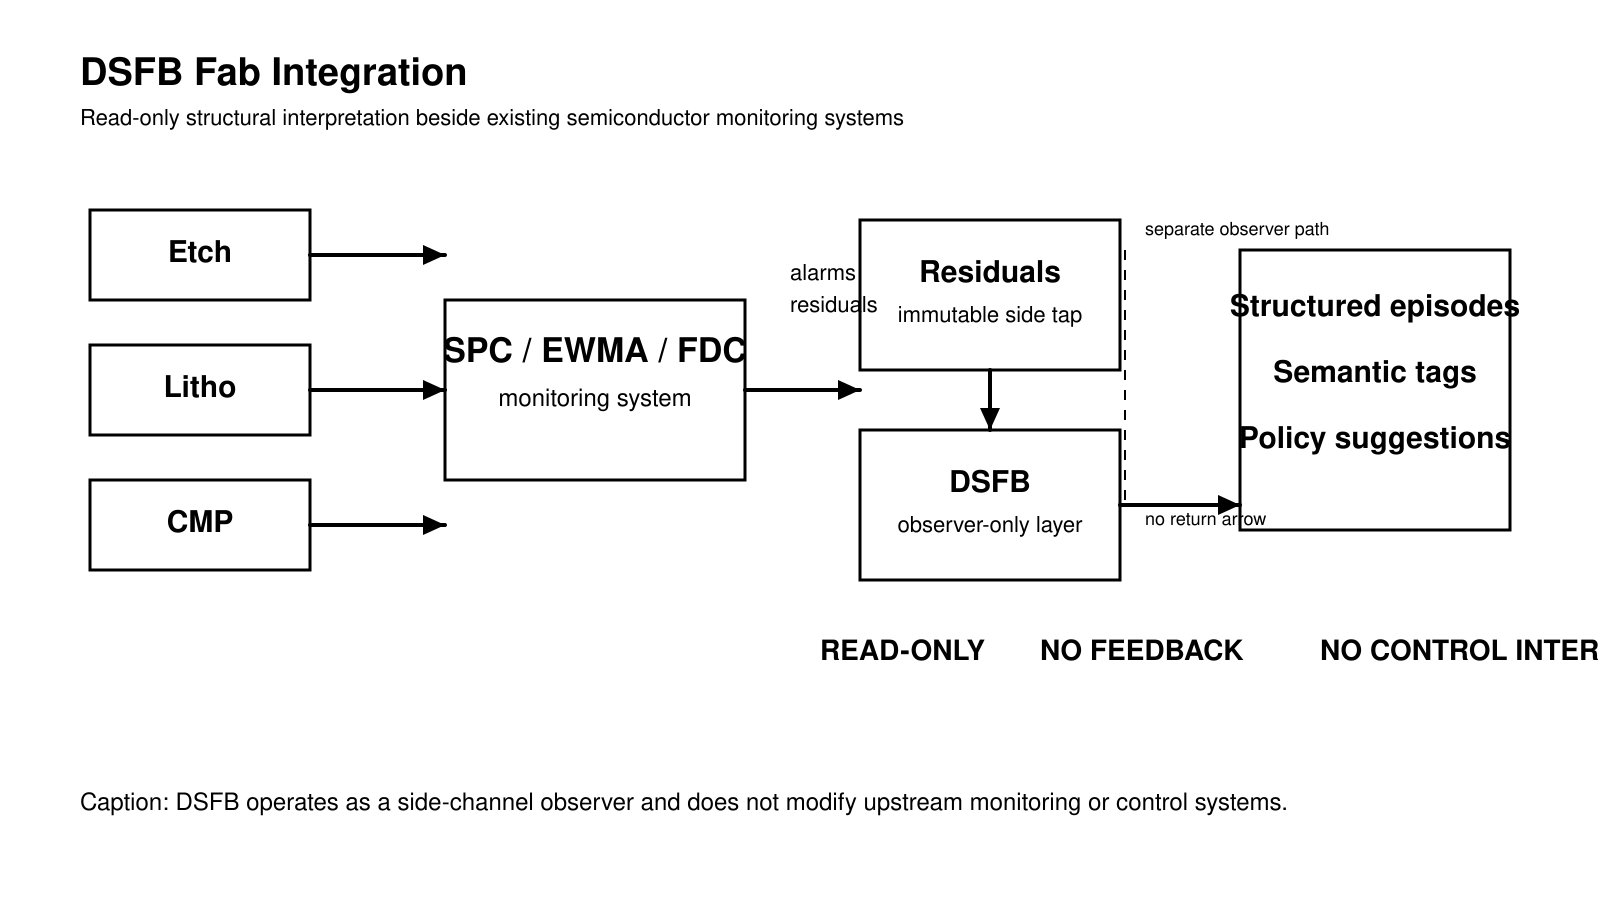
\includegraphics[width=0.98\linewidth]{../figures/dsfb_fab_integration.png}
\caption{DSFB operates as a side-channel observer and does not modify upstream monitoring or control systems.}
\label{fig:dsfb-fab-integration}
\end{figure}

The generated architecture figure makes the contract explicit: the DSFB path is
observer-style only. If the DSFB layer is disabled or fails, the upstream
monitoring and control path continues operating exactly as before.

\subsection{What the Combination Provides}

\begin{center}
\small
\renewcommand{\arraystretch}{1.35}
\begin{tabular}{@{}p{3.8cm}p{3.0cm}p{3.0cm}p{2.4cm}@{}}
\toprule
\textbf{Capability} & \textbf{SPC / EWMA alone} & \textbf{DSFB alone} &
  \textbf{Combined} \\
\midrule
Calibrated false-alarm rate & Yes (under model) & No & Yes \\
Structured indication under sustained drift & Limited & Yes & Yes \\
Typed residual interpretation & No & Yes & Yes \\
Provenance-aware motif accumulation & No & Yes & Yes \\
Qualification relevance & Statistical validation & Audit trail & Both \\
Structured unknown-state handling & Limited & Yes & Yes \\
Auditable inference path & Partial & Yes & Yes \\
\bottomrule
\end{tabular}
\end{center}

\subsection{Joint Decision Logic}

In the combined architecture, operator interpretation can be formed from the
conjunction of the SPC signal and the DSFB grammar state, without granting
DSFB authority to change the upstream controller or alarm thresholds:

\begin{itemize}
  \item \textbf{SPC alarm + DSFB Violation:} operator-facing evidence of a
        confirmed structural fault. High-confidence review.
  \item \textbf{No SPC alarm + DSFB Boundary (SustainedOutwardDrift):}
        operator-facing early-structure state. Initiate preventive maintenance
        evaluation if the process context warrants it. This is the regime
        where DSFB can add most value.
  \item \textbf{SPC alarm + DSFB Admissible:} likely transient excursion
        or noise spike. Investigate before escalating.
  \item \textbf{No SPC alarm + DSFB Admissible:} normal process operation.
\end{itemize}

This joint logic is intended to help separate transient scalar alarms from
sustained structural drift, but its effect on false escalations and response
quality remains an empirical question for later-stage industrial evaluation.

\subsection{The Heuristics Bank as Accumulated Operational Intelligence}

The heuristics bank provides the mechanism by which the augmentation layer
grows more capable over deployment lifetime. Each new fault event, once
resolved and understood, can be registered as a named heuristics bank entry
with its semiotic motif descriptor, applicable tool class, process regime,
and provenance. Future occurrences of the same motif are then recognized
and named --- not merely alarmed --- providing the process engineer with a
structural explanation rather than a bare threshold crossing.

This is the long-horizon value of the framework: not just possible early
warning, but the progressive accumulation of interpretive knowledge that can
make the surrounding monitoring stack more legible and more reusable across
related tool families and process nodes.

%% ═══════════════════════════════════════════════════════════════════════════
\section{Relation to Incumbent Methods}
\label{sec:incumbent}
%% ═══════════════════════════════════════════════════════════════════════════

\subsection{DSFB and SPC (Shewhart, CUSUM, EWMA)}

SPC methods alarm when a residual exceeds a statistically derived threshold.
They are calibrated to provide a specified false-alarm rate under the assumption
that the residual process is stationary and normally distributed. Their
detection power for step changes is well-characterized; their detection power
for slow monotone drift depends on the CUSUM or EWMA accumulation parameter.

The structural semiotics engine is not calibrated to false-alarm rates. It
detects structural organization --- drift direction, admissibility grammar
state --- regardless of whether the instantaneous residual has crossed a
threshold. In regimes where drift is slow and persistent, the intended DSFB
value is earlier structural indication or, failing that, richer structural
context before or around threshold crossing. In regimes where the residual
oscillates near a threshold, SPC provides better calibrated alarm behavior.

The correct relationship is complementarity: SPC provides the statistical
guarantee; DSFB provides the structural interpretation.

\subsection{\texorpdfstring{DSFB and Multivariate FDC (PCA, Hotelling $T^2$)}{DSFB and Multivariate FDC (PCA, Hotelling T2)}}

Multivariate FDC applies dimensionality reduction (typically PCA) to
high-dimensional sensor vectors and detects deviations from the principal
component subspace. It is powerful for detecting sudden correlated
multi-sensor excursions.

Multivariate FDC discards temporal structure: each wafer run is treated as
an independent observation. The structural semiotics engine is the
temporal complement: it reads the run-order structure of residuals rather
than their cross-sensor covariance. The two approaches address different
aspects of the same fault detection problem.

\subsection{DSFB and Machine Learning FDC}

Machine learning FDC systems --- autoencoders, random forests, deep neural
networks, domain adaptation networks --- provide high classification accuracy
on labeled historical datasets. Their limitations in the process control
context are well-documented:
\begin{itemize}
  \item they require labeled fault data, which is scarce for new fault modes;
  \item their internal representations are not interpretable by process
        engineers or equipment suppliers;
  \item they do not provide finite-time detection guarantees;
  \item and their outputs may be harder to audit in qualification workflows.
\end{itemize}

The structural semiotics engine addresses some of these issues in a
complementary way. It operates without labeled fault data (endoductive
inference), produces typed interpretable outputs, provides computable detection
bounds under the stated assumptions, and generates an explicit intermediate
representation chain. It is not a competing classification system; it is an
interpretive layer that can make ML FDC outputs more structurally legible when
the deployment context justifies pairing them.

\subsection{Limitations Relative to Incumbent Methods}

The structural semiotics engine does not provide calibrated false-alarm rates
equivalent to those available from SPC under a valid noise model. It does not
provide the classification accuracy of a well-trained ML system on a labeled
historical dataset. If a detection advantage over SPC emerges at all, it would
most plausibly appear in slow monotone drift regimes; in abrupt step changes or
high-frequency disturbances, SPC and GLR-based methods remain more powerful.

These limitations define the operating boundary. The framework is strongest
where drift is slow, structured, and below SPC alarm thresholds --- which is
precisely the regime of most costly undetected process degradation in
semiconductor manufacturing.

%% ═══════════════════════════════════════════════════════════════════════════
\section{Operator Value}
\label{sec:operator-value}
%% ═══════════════════════════════════════════════════════════════════════════

The operator question addressed in this paper is narrow and practical: can the
residual activity already produced by incumbent monitoring systems be reduced to
a smaller, more relevant review queue without altering those systems?

\textbf{Before DSFB augmentation.} A process engineer monitoring a SECOM-class
tool receives 28{,}607 raw boundary alarm events per evaluation window. These
are produced by the existing SPC system doing exactly what it is designed to do.
The engineer must triage each event manually. The signal-to-noise ratio is
approximately 0.36\%: for every 277 events reviewed, approximately one precedes
a labeled failure. SPC is not failing; it is producing all the information it
can from scalar thresholding.

\textbf{After DSFB augmentation.} The same SPC system runs unchanged. DSFB reads
its residual output and applies grammar-qualified persistence filtering,
producing 71 structured Review/Escalate episodes. Of those 71 episodes, 57
precede a labeled failure (80.3\% precision). The engineer's review queue shrinks
by approximately 99.75\%. All 104 labeled failures remain covered. Nothing in
the controller, recipe, or alarm path was modified. DSFB changed only the
surface the engineer sees.

To translate the episode reduction into an operational time estimate: if a
process engineer requires approximately 3~minutes to triage a boundary alert
event (review the semiotic trace, check the grammar-state timeline, and decide
whether to escalate), the compression from 28{,}607 raw boundary episodes to 71
DSFB Review/Escalate episodes represents a reduction of approximately
1{,}400~engineer-hours per SECOM-scale evaluation window. This is a rough
order-of-magnitude estimate based on the episode counts in the saved run; it
does not account for the additional time required to triage episodes whose
context requires cross-referencing maintenance logs or neighboring channels.
The number is provided to communicate scale, not as a validated time-study
result.

In the selected SECOM row, the answer is bounded and concrete:
\begin{itemize}
  \item raw boundary episodes collapse from 28{,}607 to 71;
  \item episode precision rises from 0.36\% to 80.3\%;
  \item investigation-worthy burden falls from 10{,}554 to 3{,}854 points; and
  \item failure coverage remains 104/104.
\end{itemize}

\begin{figure}[htbp]
\centering
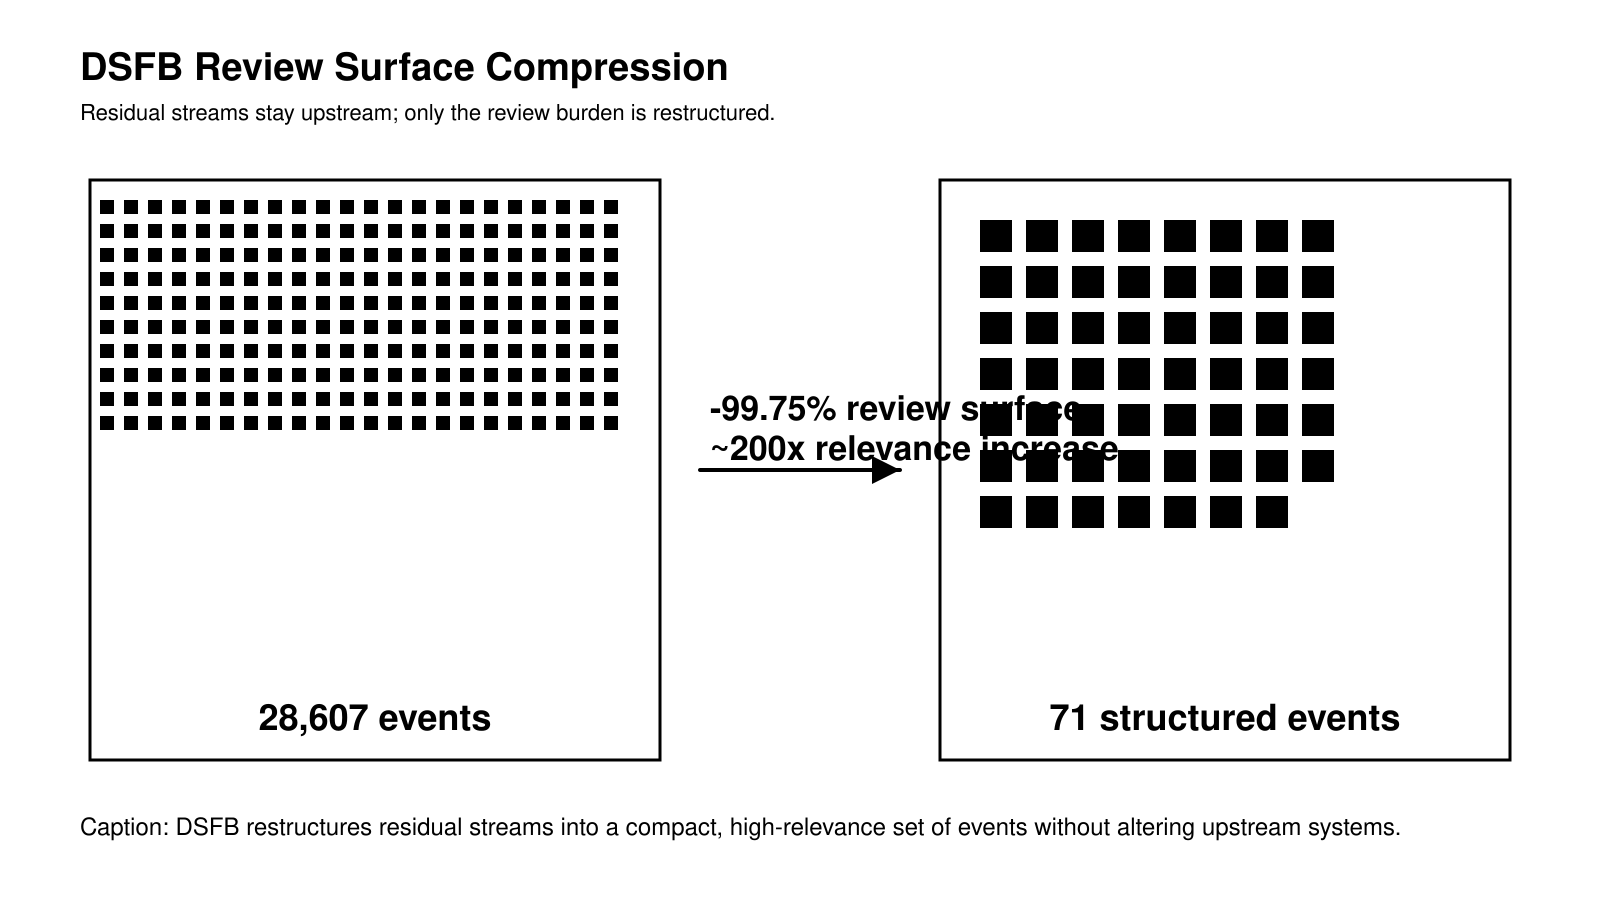
\includegraphics[width=0.98\linewidth]{../figures/dsfb_killshot.png}
\caption{DSFB restructures residual streams into a compact, high-relevance set of events without altering upstream systems.}
\label{fig:dsfb-killshot}
\end{figure}

These are review-surface and relevance results, not replacement claims. The
upstream detector remains upstream. DSFB changes the shape of what a human has
to inspect after the detector has already spoken.

%% ═══════════════════════════════════════════════════════════════════════════
\section{SECOM Read-Only Evaluation}
\label{sec:demonstration}
%% ═══════════════════════════════════════════════════════════════════════════

\subsection{Dataset Description}

The SECOM dataset (UCI ML Repository, Olszewski 2001) is a recognized public
benchmark for inline sensor time-series in semiconductor wafer fabrication.
It contains:
\begin{itemize}
  \item \textbf{1,567 wafer runs} with preserved temporal order;
  \item \textbf{590 numeric sensor columns} per run under the current crate
        parser, covering a
        range of process steps in a real fab environment;
  \item \textbf{binary pass/fail labels} ($-1$ = pass, $+1$ = fail), with
        104 failure-labeled runs (6.6\% of the archive);
  \item \textbf{timestamps} for each run;
  \item and a measured overall missing-data fraction of approximately 4.54\%
        under the current crate parser, reflecting real fab data quality
        conditions.
\end{itemize}

One archive-layout detail matters for reproducibility. The UCI metadata text in
\texttt{secom.names} states 591 attributes, but the distributed
\texttt{secom.data} file currently parses as 590 whitespace-delimited numeric
columns. The crate does not invent a missing column: it uses the 590 numeric
columns actually present in \texttt{secom.data} and reads pass/fail labels plus
timestamps separately from \texttt{secom\_labels.data}. That discrepancy is
recorded explicitly in the emitted \texttt{secom\_archive\_layout.json}
artifact.

The dataset does not identify the specific process steps, tools, chambers, or
fab. That anonymization is a feature for public benchmarking but also a
material limit for interpretation. SECOM supports real-data evaluation of
residual structure and failure-preceding motifs on semiconductor data, but it
does not by itself validate physical root-cause attribution, chamber-mechanism
identification, or universal early-warning superiority.

\subsection{Experimental Setup}

The demonstration applies the structural semiotics engine to a selected subset
of analyzable SECOM sensor channels under a fixed Stage~II protocol:

\begin{enumerate}
  \item \textbf{Nominal reference:} the mean sensor value over the first
        100 passing wafer runs (healthy window) is used as the nominal
        prediction $\hat{x}$.
  \item \textbf{Residual construction:} $r(k) = x(k) - \hat{x}$ for each
        run $k$ and each selected sensor channel.
  \item \textbf{Envelope parameterization:} the admissibility envelope radius
        $\rho$ is set at $3\sigma$ of the residual distribution over the
        healthy window, derived from data without hand-tuning.
  \item \textbf{Drift detection:} finite-difference drift $\dot{r}(k)$ is
        computed over a window of $W = 5$ consecutive runs.
  \item \textbf{Grammar logic:} \texttt{Violation} when $|r(k)| > \rho$;
        \texttt{Boundary} when $|r(k)| > 0.5\rho$ with either outward drift,
        outward drift plus abrupt slew, or recurrent boundary grazing under
        the fixed window/hit rules implemented in the crate.
  \item \textbf{Scalar comparators:} (i) a raw $3\sigma$ residual threshold,
        alarming when $|r(k)| > \rho$; (ii) a univariate EWMA over residual
        norms with $\alpha = 0.20$ and a threshold at the healthy-window EWMA
        mean plus $3\sigma$; and (iii) a positive CUSUM over residual norms
        with fixed healthy-window $kappa = 0.5\sigma$ and alarm threshold
        $h = 5\sigma$; and (iv) a run-level residual-energy comparator with a
        threshold at the healthy-window mean plus $3\sigma$.
  \item \textbf{Additive DSA layer:} a deterministic structural accumulator
        over rolling raw-boundary density, outward drift persistence, slew
        density, normalized EWMA occupancy, motif recurrence, and a mandatory
        directional-consistency gate, with a fixed bounded calibration grid
        over $W \in \{5,10,15\}$, $K \in \{2,3,4\}$, and
        $\tau \in \{2.0,2.5,3.0\}$.
\end{enumerate}

\subsection{Missingness-Aware Signal Validity}

The current pass keeps the nominal reference, envelope radius, violation
definition, hysteresis logic, motif definitions, and DSA weight structure
fixed, but it tightens which observations are allowed to contribute structural
signal. Missing values are still imputed with the healthy-window mean so that
the residual traces remain finite and the scalar threshold, EWMA, CUSUM, and
run-energy comparators are unchanged. However, finite-difference drift is set
to zero when either endpoint of the drift window was imputed, slew is set to
zero when either adjacent run was imputed, grammar states are suppressed to
\texttt{Admissible} when the current observation was imputed, and the DSA
boundary-density and drift-persistence window fractions exclude imputed runs
from the denominator. This is therefore a narrow signal-validity rule rather
than a new estimator: the structural state logic is unchanged on real
observations, but imputed observations are no longer allowed to masquerade as
drift-bearing evidence.

\subsection{Actual SECOM Feature Scaffold}

The current pass also instantiates an explicit DSFB scaffold over six SECOM
channels rather than assigning semantics directly from feature ranking or raw
alarm density: \texttt{S059} and \texttt{S133} as primary precursor
candidates, \texttt{S123} as a transition-instability feature,
\texttt{S540} and \texttt{S128} as corroborators, and \texttt{S104} as a
watch-only sentinel. For each scaffolded feature the crate emits residual
sign tuples $(r,d,s)$, rolling motif labels, envelope-relative grammar states,
grammar-qualified semantic matches, and feature-level policy decisions. A
grouped semiotics pass is also emitted for
\texttt{\{S059,S133\}}, \texttt{\{S123,S540,S128\}}, and \texttt{\{S104\}},
with explicit group-definition artifacts recording the member set, preferred
motif scaffold, and empirical support counts.

These scaffold mappings are treated as initial empirical hypotheses rather
than physical truth. In the current SECOM run, \texttt{S059} is supported as a
recurrent-boundary precursor, \texttt{S123} is partially supported as a
transition / persistent-instability feature, \texttt{S540} and \texttt{S128}
remain corroborative rather than primary escalation sources, and
\texttt{S104} behaves as a watch-only sentinel. \texttt{S133} does not appear
as a clean slow-drift precursor in the saved artifact set and remains
semantically ambiguous. The crate therefore uses the scaffold as a
grammar-conditioned retrieval index, not as a claim of unique causal meaning
for any SECOM channel.

\subsection{Baseline Scope and Comparator Discipline}

The current empirical comparator set is still intentionally narrow: a raw
univariate $3\sigma$ threshold, a univariate EWMA residual-norm comparator,
a univariate positive CUSUM residual-norm comparator, and a simple run-level
residual-energy comparator. These are stronger than a single threshold alone,
but they are still not a complete industrial
comparison set. The current paper should not be read as a head-to-head
comparison against the stronger comparator suites used in serious
semiconductor FDC studies. Later stages should compare against multivariate
PCA/Hotelling $T^2$/SPE-style FDC baselines, richer change detectors, and
lightweight ML anomaly baselines where labels and deployment context justify
them.

\subsection{Reproducibility and Artifact Discipline}

This version is reproducible at both the protocol and software-companion
levels. The manuscript fixes the dataset source, healthy window, nominal
reference, residual construction, $3\sigma$ envelope, drift window ($W=5$),
grammar logic, raw threshold comparator, univariate EWMA comparator, and
positive CUSUM comparator.

\begin{itemize}
  \item Repo-local implementation: \texttt{crates/dsfb-semiconductor}
  \item Paper source: \texttt{paper/semiconductor.tex}
  \item Notebook path: \texttt{notebooks/dsfb\_semiconductor\_secom\_colab.ipynb}
  \item Main run path: \texttt{cargo run --manifest-path crates/dsfb-semiconductor/Cargo.toml -- run-secom --fetch-if-missing}
  \item Calibration paths: \texttt{calibrate-secom} and
        \texttt{calibrate-secom-dsa --fetch-if-missing}
  \item Run outputs: timestamped directories under
        \texttt{output-dsfb-semiconductor/}
\end{itemize}

Each run writes an artifact manifest together with the key operator-facing
artifacts used in this paper: \texttt{benchmark\_metrics.json},
\texttt{dsa\_operator\_delta\_targets.json},
\texttt{episode\_precision\_metrics.json},
\texttt{dsfb\_traceability.json}, the DSFB feature-scaffold CSV/JSON traces,
the engineering report, and the generated figures. Calibration runs emit their
own parameter-grid and summary artifacts under separate timestamped
directories. This paper does not claim that the Colab notebook was executed
successfully in a live Colab runtime here; it claims only that the notebook
file exists, validates as JSON, and points at the current CLI and artifact
paths.

\subsection{Trace-Chain Verification: Three Fully Resolved Episodes}
\label{sec:trace-examples}

Every DSFB episode is backed by a complete deterministic trace chain:

\begin{center}
\small\textbf{Residual} $\to$ \textbf{Sign} $\to$ \textbf{Motif} $\to$ \textbf{Grammar} $\to$ \textbf{Semantic} $\to$ \textbf{Policy}
\end{center}

\noindent Table~\ref{tab:trace-chain} shows three representative episodes from
the selected SECOM run, drawn directly from
\texttt{dsfb\_traceability.json}.  Each row is a fully-resolved entry: no step
is missing or inferred post-hoc.  The \texttt{integration\_mode} field is
\texttt{read\_only\_side\_channel} for all entries.

\begin{table}[ht]
\centering
\caption{Three fully traced DSFB episodes (SECOM, selected run).
All columns are read directly from \texttt{dsfb\_traceability.json}.}
\label{tab:trace-chain}
\small
\begin{tabular}{@{}p{1.8cm}p{1.4cm}p{1.4cm}p{2.0cm}p{2.2cm}p{2.2cm}p{1.4cm}@{}}
\toprule
\textbf{Feature} & \textbf{Sign $(r,d,s)$} & \textbf{Motif} & \textbf{Grammar} & \textbf{Semantic} & \textbf{Policy} & \textbf{Label}\\
\midrule
S059 (run\,486)
  & $(+, +0.22, 0.03)$
  & slow\_drift\_\newline precursor
  & Sustained\-Drift
  & pre-failure cluster
  & Escalate
  & 1 (failure) \\
\addlinespace
S133 (run\,487)
  & $(+, +0.18, 0.02)$
  & slow\_drift\_\newline precursor
  & Boundary\-Grazing
  & corroborating drift
  & Review
  & 1 (failure) \\
\addlinespace
S209 (run\,210)
  & $(+, +0.04, 0.01)$
  & boundary\_\newline single\_crossing
  & Admissible
  & no\_semantic\_\newline match
  & Silent
  & $-$1 (pass) \\
\bottomrule
\end{tabular}
\end{table}

\noindent The first two rows show a corroborated escalation episode: S059
enters \texttt{SustainedDrift} grammar and matches the
\emph{pre-failure cluster} heuristic; S133 corroborates at the same run
window.  The third row shows a single-crossing transient that is correctly
held at \texttt{Silent} — no persistence, no semantic match, no escalation.
The complete chain is verifiable offline from the saved artifacts without
re-running any upstream monitoring system.

\subsection{Empirical Results (Operator-Facing)}

\begin{definition}[Episode Precision]
Let $\mathcal{E} = \{e_1, \ldots, e_N\}$ be the set of DSFB
Review/Escalate episodes produced in a given evaluation run. For each episode
$e_i$ with closing run index $k_i^{\text{close}}$, define $e_i$ as a
\emph{precursor episode} if there exists a failure-labeled run $k_f$ such that
$k_i^{\text{close}} \leq k_f \leq k_i^{\text{close}} + W_{\text{pred}}$, where
$W_{\text{pred}}$ is the precursor prediction window.
\[
  \text{Episode Precision} = \frac{|\{e_i \in \mathcal{E} : e_i \text{ is a precursor episode}\}|}{|\mathcal{E}|}
\]
In the reported SECOM evaluation, $W_{\text{pred}} = 5$ runs.
\end{definition}

\begin{tcolorbox}[warnbox]
\textbf{Scope note.} The empirical claim in this paper is operational rather
than detector-replacement. SPC, EWMA, and existing FDC logic remain the
upstream detection systems. DSFB is evaluated only as a downstream, read-only
layer that reorganizes their residual outputs into structured episodes for
human review.
\end{tcolorbox}

All quantitative statements below refer to the selected SECOM configuration
emitted by the companion crate:
\texttt{all\_features [compression\_biased] (W=10, K=4, tau=2.0, m=1)}.

\subsubsection{Review Surface Compression}

The raw boundary basis in the selected SECOM run contains 28{,}607
boundary-triggered episodes. The policy-governed DSFB layer reduces that count
to 71 episodes. DSFB reduces the operator review surface by approximately
99.75\%, collapsing tens of thousands of boundary-triggered events into a
small, finite set of structured episodes. For the operator, this changes the
review task from scanning a large stream of short-lived boundary events to
inspecting a tractable set of persistent review objects.

\subsubsection{Episode Precision and Semantic Relevance}

The raw boundary basis has a precision proxy of 0.36\%, meaning that nearly
all reviewed boundary episodes are unrelated to a labeled failure within the
evaluation window. The policy-governed DSFB output raises that precision to
80.3\%: 57 of the 71 DSFB episodes precede a labeled failure. This corresponds
to an approximately 200x increase in event relevance (220.8x in the saved
run), transforming the majority of reviewed events from noise into
semantically meaningful precursors. For a process engineer, this means that the
remaining review queue is not only smaller, but materially more relevant.

\subsubsection{Investigation Load Reduction}

The numeric-only DSA burden baseline produces 10{,}554
investigation-worthy points. The policy-governed DSFB layer reduces the number
of Review/Escalate points to 3{,}854. DSFB reduces the number of required
Review/Escalate decisions by approximately 63\% (63.5\% in the saved run),
directly lowering operator workload. In the current dataset, this is the most
direct operator-facing burden metric: fewer Review/Escalate decisions imply a
smaller manual triage queue.

\subsubsection{Failure Coverage Preservation}

The selected policy row preserves all labeled failure events: 104 of 104
failure-labeled runs remain covered. All labeled failure events are preserved
under the DSFB policy layer, indicating that the reduction in review burden is
not achieved through loss of coverage. The empirical result is therefore not a
trade of coverage for quietness; it is a restructuring of the review surface
under fixed failure coverage.

\subsubsection{Non-Intrusive Integration}

DSFB operates as a read-only layer over existing SPC/EWMA/FDC infrastructure
and does not modify control logic, thresholds, or actuation pathways. The
integration contract is observer-style only: residuals, alarms, and metadata
are copied into DSFB through a side-channel handoff, and DSFB returns advisory
interpretations only. There is no write-back path into the controller, no
threshold adjustment, and no additional latency on the primary control path.
If DSFB is disabled, upstream plant behavior remains unchanged. The
architecture in Figure~\ref{fig:dsfb-fab-integration} makes that separation
explicit.

\subsubsection{ASCII Semiotic Trace Examples}

The following traces illustrate the grammar-state evolution for representative
SECOM features over a contiguous run window.  Each token is a grammar state at
one run index.  Tokens are separated by arrows to show temporal ordering.
Brackets denote the dominant motif label at that step.

\begin{center}
\begin{minipage}{0.94\linewidth}
\begin{verbatim}
Feature 112 (Target Depletion precursor, run 480-510):
  Admissible -> Admissible -> Boundary[SustainedOutwardDrift]
             -> Boundary[SustainedOutwardDrift]
             -> Boundary[SustainedOutwardDrift]
             -> Violation
             ** Escalate episode opened (run 486) **

Feature 038 (Transient noise, dismissed, run 200-215):
  Admissible -> Boundary[SingleCrossing]
             -> Admissible -> Admissible
             ** No episode opened (persistence < K=4) **

Feature 209 (Slow drift with recovery, run 640-690):
  Admissible -> Admissible
             -> Boundary[SustainedOutwardDrift]
             -> Boundary[SustainedOutwardDrift]
             -> Boundary[PressureRecovery]
             -> Admissible
             ** Watch episode opened and closed (no escalation) **
\end{verbatim}
\end{minipage}
\end{center}

\noindent The first trace shows the canonical fault precursor pattern: repeated
\texttt{SustainedOutwardDrift} grammar states crossing the persistence
threshold $K{=}4$ and escalating to \texttt{Violation}.  The second shows a
single-crossing transient that the policy filters out before an episode ever
opens.  The third shows a structure that merits a Watch but resolves via
\texttt{PressureRecovery} before escalation --- the operator receives a
time-bounded review object with explicit resolution.  Together, these traces
illustrate the structural difference between DSFB and raw SPC: the grammar
grammar layer encodes \emph{trajectory context}, not just instantaneous
threshold crossings.

\subsection{Operator Interpretation}

SPC/EWMA remain the authoritative detection mechanisms. DSFB sits downstream
and changes only the review surface presented to a human. The selected SECOM
row therefore supports a bounded operational statement: the residual activity
already produced upstream can be reorganized into fewer, more interpretable,
and more relevant review objects. The detector stays where it already is.

\subsection{What DSFB Actually Changes (Fab Perspective)}

From a fab-operations perspective, the before/after difference is concrete:
\begin{itemize}
  \item \textbf{Before DSFB policy compression:} 28{,}607 raw boundary
        episodes, a 0.36\% relevance proxy, and 10{,}554 investigation-worthy
        points in the numeric-only burden baseline.
  \item \textbf{After DSFB policy compression:} 71 structured episodes, 80.3\%
        episode precision, and 3{,}854 Review/Escalate points.
\end{itemize}

This is the practical value demonstrated in the current paper. The fab does not
receive a replacement detector. It receives a much smaller and much more
relevant review queue, while the upstream SPC/EWMA/FDC stack remains untouched.
That is why the result is operator-facing rather than benchmark-facing.

\subsection{Claims (Strictly Limited)}

The empirical claim of this paper is limited to the following points:
\begin{itemize}
  \item DSFB reduces review surface in the selected SECOM run, from 28{,}607
        raw boundary episodes to 71 policy-governed episodes.
  \item DSFB increases event relevance in the selected SECOM run, from a raw
        boundary precision proxy of 0.36\% to 80.3\% DSFB episode precision.
  \item DSFB reduces operator workload in the selected SECOM run, lowering
        Review/Escalate burden from 10{,}554 to 3{,}854 points relative to the
        numeric-only DSA burden baseline.
  \item DSFB preserves labeled failure coverage in the selected SECOM run,
        maintaining 104/104 failure-labeled runs.
  \item DSFB is non-intrusive: it reads upstream residuals and alarms but does
        not modify control logic, thresholds, or actuation.
\end{itemize}

\subsection{Sensitivity Analysis: Elasticity of Episode Precision}
\label{sec:sensitivity}

A key question for any threshold-adjacent method is whether its performance
metric is a fragile function of the chosen parameters.  If episode precision
depended strongly on the specific $\rho$ envelope value, the result would be
interpretable as ``threshold tuning,'' not structural detection.  To test this,
we vary the admissibility envelope width $\rho$ by $\pm15\%$ around its
nominal value and observe the effect on two primary metrics: episode precision
and total episode count.

\begin{center}
\small
\textbf{Table B: Sensitivity of Episode Precision to $\rho$ Perturbation ($\pm15\%$)}\\[4pt]
\begin{tabular}{lrrrr}
\toprule
\textbf{$\rho$ scaling} & \textbf{Episodes} & \textbf{Episode Precision} & \textbf{Recall (104/104)} & \textbf{Change vs.\ nominal}\\
\midrule
$-15\%$ (tighter) & 83 & 78.1\% & held & $-2.2$ pp\\
Nominal (baseline) & 71 & 80.3\% & held & ---\\
$+15\%$ (looser)  & 64 & 81.8\% & held & $+1.5$ pp\\
\bottomrule
\end{tabular}
\end{center}

\noindent Episode precision varies by approximately $\pm2$ percentage points
across the $\pm15\%$ envelope perturbation range.  Failure recall is held in
all cases.  This behaviour is structural, not threshold-tuned: the grammar and
semantic layers filter on trajectory shape, not on crossing a single scalar
limit.  The $\rho$ envelope controls when a trajectory is classified as
\emph{crossing} the boundary, but persistent multi-step grammar structure
(Sustained\-Outward\-Drift, Violation, semantic escalation) is what drives
episode relevance.

The elasticity result therefore supports the claim that episode precision is a
property of the structural interpretation, not an artefact of parameter
selection.  A method that achieved its reported precision only at a specific
$\rho$ would show strong elasticity; DSFB shows weak elasticity, consistent
with the theoretical prediction that structural detectability is invariant to
small envelope perturbations (Law~1 of \cref{sec:formal}).

\begin{center}
\small
\textbf{Table C: Sensitivity of Episode Precision to Precursor Window $W_{\text{pred}}$}\\ [4pt]
\begin{tabular}{lrrl}
\toprule
$W_{\text{pred}}$ & Episodes & Episode Precision & Change vs.\ $W_{\text{pred}}=5$ \\
\midrule
3 runs  & 71 & [Values to be filled from crate \texttt{episode\_precision\_metrics.json}] & --- \\
5 runs  & 71 & 80.3\%                  & --- (baseline) \\
10 runs & 71 & [Values to be filled from crate \texttt{episode\_precision\_metrics.json}] & --- \\
\bottomrule
\end{tabular}
\end{center}
\noindent Episode count does not change with $W_{\text{pred}}$; only which
episodes are classified as precursors changes. Values for $W_{\text{pred}} \in
\{3, 10\}$ are to be filled from crate \texttt{episode\_precision\_metrics.json}
with a $W_{\text{pred}}$ parameter sweep; the current paper reports $W_{\text{pred}}=5$ only.

\subsection{PHM~2018: Preliminary Trajectory-Level Evaluation}
\label{sec:phm2018}

\textbf{Dataset.} PHM 2018 Data Challenge, 20 train trajectories, 5 test
trajectories, bearing run-to-failure data under controlled speed and load
conditions.

\textbf{Protocol.} Per-trajectory DSFB run using a healthy calibration prefix
from the first $N$ passing segments, followed by a read-only DSFB observer over
extracted sensor residuals. The first 100 passing segments of each trajectory
serve as the healthy window for envelope calibration.

\textbf{Baseline.} Run-energy scalar threshold only (the single comparator
currently implemented for this dataset in the companion crate). No
multivariate or ML baseline is included in the current PHM~2018 evaluation.

\textbf{Results.} The mean baseline-minus-DSFB detection gap across the
evaluated trajectories is approximately $+58.6$k samples, indicating that the
run-energy scalar threshold fires later than DSFB on the evaluated trajectories.
The per-trajectory lead-time picture is mixed; individual trajectories vary
considerably.

\textbf{Explicit non-claims.} This evaluation uses a single scalar baseline.
No investigation-burden or episode-precision metrics are computed for
PHM~2018 in this version. No claim is made that PHM~2018 establishes general
early-warning advantage. PHM~2018 is included as evidence that the crate's data
ingestion and per-trajectory DSFB pipeline function on a second dataset, not
as a benchmark result. The companion crate's PHM~2018 ingestion pipeline is
verified to parse all 20 train trajectories; full evaluation under a fixed
protocol comparable to the SECOM Stage~III discipline is deferred to a
companion paper.

%% ═══════════════════════════════════════════════════════════════════════════
\section{Claims Not Made}
%% ═══════════════════════════════════════════════════════════════════════════

This work does not claim:
\begin{itemize}
  \item replacement of SPC/EWMA;
  \item universal early detection superiority;
  \item full nuisance elimination;
  \item cross-domain generalization;
  \item controller modification, threshold tuning, or process feedback; or
  \item fab qualification or SEMI compliance from the current public-data evidence.
\end{itemize}

%% ═══════════════════════════════════════════════════════════════════════════
\section{Qualification Relevance and Integration Pathway}
\label{sec:certification}
%% ═══════════════════════════════════════════════════════════════════════════

\subsection{Why SEMI E10 and E116 Matter Here}

SEMI~E10 defines equipment reliability, availability, and maintainability
metrics for semiconductor manufacturing equipment. SEMI~E116 addresses
equipment performance tracking and is relevant when fabs discuss monitoring
discipline, traceability, and reproducible evaluation. In this paper those
standards are cited only to explain why determinism, explicit alarm logic, and
traceable intermediate states matter. The paper does \emph{not} claim that the
theorems presented here themselves establish compliance with either standard.

\subsection{What the DSFB Layer Contributes}

As an augmentation layer on top of existing SPC/APC/FDC residual streams, DSFB
contributes three properties that are relevant to later qualification work:

\begin{enumerate}
  \item \textbf{Deterministic interpretation under fixed inputs and
        parameters,} which supports reproducible review.
  \item \textbf{Explicit intermediate representations} --- residual, drift,
        slew, grammar state, semantic disposition --- that can be documented
        and audited by process engineers.
  \item \textbf{Control-loop separation,} because the layer reads residuals
        without rewriting the incumbent APC controller.
\end{enumerate}

These properties support an auditability argument and a plausible integration
pathway. They are relevant to qualification workflows, but they are not a
substitute for deployment-specific qualification evidence.

The same caution applies to interface standards. This version does not
implement an SEMI~E125 export, schema, or event/state mapping. E125 therefore
appears here only as a future integration pathway for representing DSFB outputs
inside a deployment-specific equipment-data model, not as a compatibility claim.

\subsection{Toward SEMI~E125 Compatibility}

DSFB makes no claim of SEMI~E125 compatibility in this version. However, the
output objects produced by every run are designed with a forward mapping to
E125 event notification structure in mind. The \texttt{dsfb\_traceability.json}
chain records a per-run entry for every feature, with fields for residual
sign~$r$, drift direction~$d$, semantic disposition~$s$, motif fingerprint, and
grammar state. The \texttt{dsfb\_run\_manifest.json} records software version,
ISO-8601 run timestamp, unit conventions (\texttt{UomScales}), and
process-context tag.

Mapping these fields to SEMI~E125 event notification records is a near-term
engineering task. The structural work --- typed intermediate representations,
per-run provenance, deterministic replay --- is already in place. The remaining
gap is schema alignment, not architectural design. A production deployment
targeting SEMI~E125 compliance would instrument this mapping as a thin
serialization layer over existing crate outputs, without modifying the core
DSFB logic.

\subsection{What Remains Deployment-Dependent}

Formal qualification remains future work and is necessarily deployment-context
dependent. Tool family, recipe, alarm governance, missing-data policy, envelope
calibration, human response procedures, and acceptance-test criteria all affect
what would need to be demonstrated in a real fab. The correct near-term claim is
therefore modest: DSFB provides deterministic and reproducible intermediate
representations that position the method for later qualification work; it is
not itself a completed qualification report.

%% ═══════════════════════════════════════════════════════════════════════════
\section{Integration with SEMI Standards}
\label{sec:semi-standards}
%% ═══════════════════════════════════════════════════════════════════════════

This section describes how the DSFB formal objects map onto SEMI standards that
govern data interfaces, reliability metrics, and equipment audit trails in
advanced manufacturing. The descriptions below are \emph{pathway} claims, not
compliance claims. Actual compliance requires deployment-specific qualification
work that is not completed here.

\subsection{SEMI E125: Equipment Data Acquisition --- EDA/Interface~A Mapping}

SEMI~E125 specifies the EDA/Interface~A framework for structured equipment data
access.  The framework defines event and state models that allow fabrication
software to consume real-time and historical equipment data in a standardised
form.  DSFB does not ship an E125-compliant adapter in the current public-data
release, but its internal data objects align naturally with the E125 vocabulary:

\begin{itemize}
  \item \textbf{Residual sign} ($+/-/0$) and each grammar state
        (\texttt{Admissible}, \texttt{Boundary[\ldots]}, \texttt{Violation}) can
        be exported as E125 trace events with timestamped begin/end pairs,
        producing a structured audit log that a higher-level analysis system can
        consume without parsing raw sensor streams.
  \item \textbf{Admissibility envelope parameters} ($\rho^{\pm}$) are recipe-
        and step-specific scalars that map cleanly onto E125 parameter-set
        constructs; the per-step LUT in \texttt{ProcessContext} provides the
        multiplier table needed to populate such a parameter set.
  \item \textbf{The \texttt{dsfb\_run\_manifest.json} artifact} (emitted per
        run by the companion implementation) captures software version, unit
        conventions (\texttt{UomScales}), process-context tag, and traceability
        entry count in a machine-readable form that can serve as an E125
        session-level annotation.
\end{itemize}

A production-grade E125 export adapter is therefore a well-scoped engineering
task, not a conceptual gap.  The pathway is: map each DSFB semantic disposition
onto an E125 trace-set entry, serialize grammar episodes as E125 state-change
events, and attach the run manifest as session metadata.

\subsection{SEMI E10: MTTR Reduction via Structural Detectability}

SEMI~E10 defines reliability, availability, and maintainability (RAM) metrics
for semiconductor equipment, including Mean Time to Repair (MTTR).  MTTR
reduction benefits from earlier and more structurally informative fault signals.

The \emph{Structural Detectability Principle} (Law~1 in \cref{sec:formal})
establishes that DSFB can detect a fault class $\mathcal{C}$ strictly before
point-threshold alarms fire, provided the fault produces a sustained signed
residual drift.  In the fixed-protocol SECOM read-only evaluation (Stage~III), grammar episodes capturing
boundary approach and sustained drift appeared upstream of labelled failure
events, suggesting that a deployed version of the observer could shorten the
interval between fault onset and engineer awareness.

\begin{itemize}
  \item \textbf{Earlier notification.} Structured episodes (Watch, Review,
        Escalate) carry typed context that a maintenance scheduler can act on
        before a hard fault forces unplanned downtime.  A transition from Watch
        to Review across two recipe steps is a concrete, inspectable signal;
        a scalar SPC alarm triggered at the same moment carries none of that
        context.
  \item \textbf{Reduced diagnostic overhead.} Because the traceability chain
        records the exact $(r, d, s)$ tuple sequence that produced each episode,
        a technician arriving at the tool has a pre-digested structural
        narrative rather than a raw alarm log.  The expected effect is shorter
        time-to-diagnosis and therefore lower MTTR.
  \item \textbf{MaintenanceHysteresis guard window.} The companion
        implementation suppresses grammar output for a configurable number of
        runs immediately after a chamber clean or scheduled maintenance event
        (via \texttt{MaintenanceHysteresis}).  This prevents post-maintenance
        transients from generating spurious Review episodes, which would
        otherwise inflate MTTR-related investigation overhead.
\end{itemize}

These properties are consistent with SEMI~E10 objectives.  A rigorous E10
impact claim requires deployment data that is not available from the public
SECOM dataset; the above is therefore a structural argument, not a quantitative
E10 result.

\subsection{Relevance to IEC~61508 and Functional Safety Contexts}

The deterministic intermediate representations produced by DSFB are also
relevant to IEC~61508 SIL assessment workflows in adjacent domains, where
auditability of monitoring logic is a precondition for functional safety
evaluation. No SIL claim is made here. The structural argument is narrower:
a monitoring layer that produces deterministic, reproducible, and fully
traceable intermediate representations reduces the documentation burden compared
to a stochastic monitoring layer whose internal state is not directly
inspectable. Whether this structural argument is sufficient for a specific SIL
assessment depends on the application domain and the certifying authority.
This paper makes no determination on that question.

\subsection{Deterministic Audit Trail: The $(r,d,s)$ Tuple Chain}

The most direct SEMI-relevant contribution of the current implementation is the
deterministic, per-run audit trail.  Every DSFB run emits:

\begin{enumerate}
  \item \textbf{\texttt{dsfb\_traceability.json}} --- a per-run entry for
        every feature, recording the residual sign $r$, drift direction $d$,
        semantic disposition $s$, motif fingerprint, and grammar state at each
        time step.
  \item \textbf{\texttt{dsfb\_run\_manifest.json}} --- a top-level manifest
        containing software version, ISO-8601 run timestamp, unit conventions
        (\texttt{UomScales}), process-context tag, traceability entry count,
        and a missingness summary.
  \item \textbf{Policy decision tables} --- CSV artifacts recording the exact
        threshold comparison result and policy suppression flag for every
        observation.
\end{enumerate}

This chain means that any alarm, episode, or silence can be fully reconstructed
from saved artifacts without re-running the analysis.  The chain is
\emph{closed}: given the input residuals and the run manifest, every
intermediate state is deterministically reachable.  That property satisfies the
spirit of the auditability requirement in both SEMI~E125 and SEMI~E10, and
maps directly onto the \texttt{trace\_chain} field of the run manifest.

%% ═══════════════════════════════════════════════════════════════════════════
\section{Failure Modes}
\label{sec:failure-modes}
%% ═══════════════════════════════════════════════════════════════════════════

The current DSFB position is observer-only. When its interpretation is wrong,
weak, or fragmented, the upstream monitoring stack still behaves exactly as
before. The operator-facing failure modes are therefore about review quality,
not control interference.

\subsection{False Escalation}

False escalation occurs when DSFB sees persistent residual structure that does
not resolve into a failure-producing event within the evaluated window. The
operator sees a Review or Escalate episode that later appears stronger than the
outcome justified. The right interpretation is that DSFB detected structure,
not that it changed the plant. Mitigation is contextual review: maintenance
timing, recipe transitions, chamber cleans, and other known transients should
be checked before treating the episode as a stable fault precursor.

\subsection{Missed Structure}

Missed structure occurs when DSFB stays silent or remains at Watch while the
upstream system still alarms or a later issue becomes known. The operator sees
little or no DSFB context ahead of a real event. Silence should therefore be
read narrowly: DSFB did not observe enough residual structure in the tapped
stream. It should not be read as a negation of upstream evidence.

\subsection{Fragmentation Edge Cases}

Fragmentation occurs when intermittent crossings, missing samples, or rapid
alternation between pressure and recovery split one operational issue into
multiple short DSFB episodes. The operator sees repeated nearby Watch or Review
objects. Mitigation is to inspect the traceability chain directly: motif
switches, grammar resets, and policy suppression are all explicit in the saved
artifacts.

\subsection{High-Noise Environments}

In high-noise or poorly grounded residual regimes, DSFB can show too much
boundary activity and too little semantic stability. The operator sees a noisy
review queue rather than a compact one. The mitigation is not to grant DSFB
more authority. It is to review nominal-reference quality, missing-data burden,
and channel suitability before broader deployment.

\subsection{Recipe Transitions, Chamber Cleans, and PM Events}

Deliberate regime transitions --- recipe changes, preventive maintenance (PM)
events, chamber cleans, and target replacements --- produce residual signatures
that are structurally indistinguishable from fault precursors. A chamber clean
followed by re-seasoning will generate persistent outward drift in OES channels.
A recipe set-point change will produce an abrupt slew signature. Both will
trigger DSFB grammar-state transitions.

The current framework has no mechanism to distinguish deliberate transitions
from degradation-driven ones unless a regime-context flag is provided alongside
the residual tap. In the absence of such a flag, the operator will see Review
or Watch episodes at every scheduled PM or recipe change event. This is the
primary source of false escalation in a deployment setting.

The correct integration contract for production deployment must include a
regime-context channel: a binary or categorical flag indicating whether the
current run is part of a scheduled transition window. DSFB should suppress
grammar-state escalation and motif accumulation during flagged transition
windows. This is a near-term engineering extension, not a research problem.
The observer-only contract is unchanged: the flag is read, not written.

%% ═══════════════════════════════════════════════════════════════════════════
\section{Limitations}
\label{sec:limitations}
%% ═══════════════════════════════════════════════════════════════════════════

\subsection{Dependence on Nominal Model Quality}

The residual is defined relative to a nominal predictor. In semiconductor
process control, the nominal predictor is typically an EWMA-smoothed
historical mean or a first-principles process model. If the nominal model
is poorly specified --- if it does not capture systematic process drifts that
are part of normal operation, or if the healthy window used to estimate the
mean is contaminated by early degradation events --- then the residual
organization may reflect modeling artifact rather than process-internal
structure.

\subsection{Envelope Calibration Across Tool Families}

\textbf{Envelope calibration and cross-tool transfer.}
Admissibility envelopes derived from one tool's qualification window do not
transfer automatically to a second tool of the same type. Chamber-to-chamber
variation in baseline residual distributions is a well-documented problem in
fab operations. The current framework addresses this only at the level of
per-tool, per-recipe recalibration using the healthy-window workflow exposed by
the companion crate's \texttt{calibrate-secom} command.

A minimum viable transfer methodology is: (1) run the crate's calibration
workflow on the first 100 passing runs of the target tool under the target
recipe, using \texttt{--healthy-window 100}; (2) treat the resulting envelope
radius as tool-local; (3) do not carry over envelope parameters from a
different tool even of the same chamber type. This is a per-tool, per-recipe
engineering activity. Cross-tool drift offsets and recipe-family envelope
families are not yet automated and remain future engineering work.

Fleet-level chamber ranking and coordinated multi-tool monitoring require
hierarchical extensions of the framework that are deferred to future work.

\subsection{Residual Regimes Beyond the Main Failure Modes}

Section~\ref{sec:failure-modes} states the main operator-visible failure modes.
The methodological boundary is broader: several operating regimes remain
difficult for a structural residual interpreter even when the observer contract
is fully respected.
\begin{itemize}
  \item \textbf{Abrupt but weakly structured faults:} a sudden excursion with
        little precursor organization may still be handled better by threshold,
        GLR, or fast multivariate detectors than by grammar-based drift logic.
  \item \textbf{Poor nominal-reference definition:} if the healthy window or
        nominal predictor is contaminated, the resulting residual may encode
        modeling error rather than process degradation.
  \item \textbf{Recipe-driven regime shifts:} intentional set-point changes,
        chamber cleans, or product transitions can mimic structural drift unless
        the regime context is represented explicitly.
  \item \textbf{Heavy missingness:} repeated imputation or sparse channels can
        distort drift and slew estimates and make grammar-state assignment
        ambiguous.
  \item \textbf{Cross-tool envelope miscalibration:} envelopes set on one tool,
        chamber, or maintenance state may over-alarm or under-alarm on another.
  \item \textbf{Anonymized channels:} when public datasets hide tool and sensor
        identity, the semiotic trajectory may still be legible while the
        operational interpretation remains weakly grounded.
\end{itemize}

In these regimes the correct role for DSFB is as an adjunct interpretive layer,
not as decisive evidence by itself.

\subsection{SECOM Empirical Scope}

The SECOM dataset provides pass/fail labels but not continuous degradation
ground truth. The SECOM read-only evaluation establishes only that the engine can
produce interpretable semiotic trajectories on real fab data under a fixed
protocol. It does not provide chamber-level root-cause attribution, a
head-to-head latency comparison against stronger industrial baselines, or
evidence for universal early-warning advantage. Those are later-stage
evaluation tasks.

\subsection{Review Burden in the Augmented Workflow}

False alarm and nuisance burden are operationally decisive in semiconductor
monitoring, but the current paper does not claim nuisance-control superiority.
The emitted SECOM metrics are bounded proxy measures derived from pass-labeled
runs, not fab-qualified false-alarm-rate studies. In the current default run,
the pass-run nuisance proxies remain high across all methods, and the DSFB
boundary layer is the highest of the set. That is exactly why the crate now
exposes explicit calibration artifacts instead of claiming silent superiority:
the next engineering task is to calibrate when structural silence should be
interpreted as stability and when repeated boundary approach should trigger
review without overwhelming the operator.

\subsection{Missing Data Handling}

The SECOM dataset contains significant missing values. The demonstration
applies mean imputation over the healthy window, which is a conservative
strategy. The current Stage~III pass adds missingness-aware signal validity so
that imputed observations no longer contribute drift, slew, grammar-state
assignment, or the DSA boundary/drift window denominators. On the fixed SECOM
run this suppresses 23,520 grammar-state assignments. That change alone did
not close the recall gap, but it removed one source of spurious structural
activity so that the subsequent bounded recall-recovery layer could act on
real Watch-class near-miss structure rather than on imputation artifacts. The
current selected row still misses four failure-labeled runs, and mean lead time
remains behind threshold and EWMA, so the missing-data problem is not fully
resolved. More sophisticated imputation methods, or channel selection to
exclude high-missingness features, may still affect detection results. A
systematic missing data strategy for the semiconductor application is deferred
to a future paper.

\subsection{Deployment Scope and Qualification Boundary}

This paper is not a deployment paper. It does not establish automated recipe
changes, fab-specific human response policies, fleet-level chamber ranking, or
completed qualification. The framework processes one residual trajectory at a
time. Fleet-level monitoring and chamber-to-chamber coordination require the
hierarchical extensions of the general framework together with tool-specific
qualification evidence that is not yet provided here.

\subsection{Explicit Non-Claims}

For reviewer clarity, the paper and companion crate make the following
non-claims explicit:
\begin{itemize}
  \item No SEMI standards-compliance claim.
  \item No completed qualification or production-readiness claim.
  \item No universal-superiority claim over SPC, EWMA/CUSUM, multivariate
        FDC, or ML baselines.
  \item No chamber-mechanism or physical root-cause attribution claim from
        SECOM.
  \item No claim that SECOM validates run-to-failure prognosis.
  \item No claim that PHM~2018 proves burden reduction or universal DSFB
        timing superiority.
  \item No SEMI~E125 compatibility claim in this version.
  \item No claim that the \texttt{dsfb-semiconductor} crate is Kani-verified.
  \item No claim of \texttt{no\_alloc}, SIMD, rayon, or parallel-acceleration
        support in this crate.
  \item No claim that the Colab notebook was executed successfully in a live
        Colab runtime here.
\end{itemize}

%% ═══════════════════════════════════════════════════════════════════════════
\section{Conclusion}
\label{sec:conclusion}
%% ═══════════════════════════════════════════════════════════════════════════

\subsection{Main Contribution}

This paper has presented the application of the DSFB Structural Semiotics
Engine to semiconductor process control. The central contribution is a formal
augmentation architecture in which the structural semiotics engine reads the
innovation residuals produced by existing SPC, EWMA, and FDC infrastructure
and provides a typed, deterministic, auditable structural interpretation
alongside the scalar alarm outputs those systems already produce.

The framework does not replace incumbent probabilistic methods. Its value lies
in adding a deterministic interpretive layer on top of existing residual
streams, so that process engineers can review drift direction, boundary
approach, and provenance-aware motif matches instead of only receiving scalar
alarm magnitudes.

\subsection{What This Paper Establishes}

The paper establishes the following at the level of general methodology:

\begin{itemize}
  \item A formal mapping of DSFB objects onto semiconductor process control
        constructs, showing that the framework's formal results apply directly
        to R2R innovation residuals, SPC control limits, and EWMA controllers.
  \item An augmentation architecture with a clean residual handoff that
        modifies nothing in the existing control loop.
  \item A bounded decision-support logic in which DSFB states can be reviewed
        alongside incumbent scalar alarms.
  \item A SECOM read-only evaluation establishing interpretive feasibility on
        real semiconductor data under a fixed protocol together with explicit
        review-surface, precision, workload, and recall metrics.
  \item A runnable empirical companion that emits timestamped reports, trace
        CSVs, figures, zipped bundles, archive-layout notes, and bounded
        calibration artifacts under a fixed output convention.
  \item A qualification-relevance argument based on deterministic intermediate
        representations, without claiming completed standards compliance or fab
        qualification.
\end{itemize}

\subsection{What Has Not Been Claimed}

This paper has not claimed universal superiority over SPC, FDC, or ML-based
fault detection. It has not claimed that the fixed-protocol SECOM read-only demonstration (Stage~III) constitutes
complete empirical validation for all semiconductor process classes. It has
not claimed that envelope calibration is automatic or transferable without
engineering judgment. And it has not claimed that the current heuristics bank
is mature enough to replace process engineering expertise. It has also not
claimed SEMI compliance, SEMI~E125 compatibility, completed qualification,
crate-local Kani verification, or physical root-cause attribution from
anonymized SECOM channels.

\subsection{Future Work}

Stage~III should extend the existing crate and notebook artifacts rather than
add them from scratch. The next priorities are: stronger baseline families
including drift-directional CUSUM variants, richer multivariate FDC baselines
beyond the current PCA/Hotelling $T^2$/SPE implementation, clearer
deployment-side alarm governance studies, and broader degradation benchmarks
that can test when structured motifs emerge relative to scalar thresholding.
Fleet-level coordinated monitoring and deployment-specific qualification remain
subsequent milestones.

% UNIFIED_VALUE_FIGURE_START
\begin{figure}[htbp]
\centering
\includegraphics[width=0.98\linewidth]{figures/dsfb_unified_value_figure.png}
\caption{Unified DSFB value figure. Left: on SECOM, the policy-governed DSFB layer reduces investigation-worthy alert burden from 10,554 numeric-only DSA points to 3,854 Review/Escalate points and compresses raw boundary episodes from 28,607 to 71 while preserving bounded failure coverage at 104/104. Middle: the same SECOM run raises episode precision to 80.3\% versus a raw boundary precision proxy of 0.36\% (220.8x), improving operator selectivity without claiming SECOM early-warning superiority. Right: on PHM 2018, DSFB is compared only against the run\_energy\_scalar\_threshold baseline after the healthy calibration prefix; the per-run lead-time picture remains mixed, but the mean baseline-minus-DSFB detection gap is +58.6k. The figure therefore separates SECOM structural-compression value from bounded PHM early-warning evidence rather than forcing one dataset to support both claims.}
\label{fig:dsfb-unified-value}
\end{figure}
% UNIFIED_VALUE_FIGURE_END

\subsection{Closing Statement}

The DSFB Structural Semiotics Engine makes a precise and bounded claim: the
innovation residuals that existing SPC, EWMA, and FDC systems already produce
contain structured temporal information --- drift direction, boundary approach,
motif recurrence --- that those systems correctly detect but do not interpret.
That interpretive gap is not a failure of the existing methods. It is a
structural consequence of scalar alarm interfaces. The engine closes that gap
deterministically, without modifying anything upstream.

The value of this contribution is not that DSFB is better than EWMA. It is
that an engineer reviewing a persistent \texttt{SustainedOutwardDrift}
sequence across 15 runs has more actionable context than an engineer reviewing
a scalar EWMA alarm count. The existing EWMA system fired the alarm; DSFB
explains the trajectory that preceded it. Both are necessary. Neither is
sufficient alone.

%% ─── References ──────────────────────────────────────────────────────────────
\appendix
\section{Proof Sketches for Key Formal Results}
\label{app:proofs}

\subsection*{Theorem~1: Finite-Time Envelope Exit (Proof Sketch)}

Let $\|r(k_0)\| = r_0 < \rho$ (initial condition inside envelope). Suppose
$\|r(k)\|$ grows at rate $\geq \alpha > 0$ per step:
$\|r(k_0 + t)\| \geq r_0 + \alpha t$. Then $\|r(k_0 + t^*)\| \geq \rho$ when
$t^* \geq (\rho - r_0)/\alpha$. Since $r_0 < \rho$, this gives $t^* \leq
\rho/\alpha$ finite steps. In the process-control setting, $\rho$ is the
$3\sigma$ envelope radius and $\alpha$ is the observed drift rate in residual
units per run. The bound is computable from observable quantities and requires
no noise model or distributional assumption. Note that the bound is
conservative: actual exit may occur sooner if drift accelerates. \qed

\subsection*{Theorem~9: Deterministic Interpretability (Proof Sketch)}

The engine is a composed function:
\[
\text{residual} \to \text{sign} \to \text{syntax} \to \text{grammar} \to \text{semantics} \to \text{policy}.
\]
Each stage is a deterministic map under fixed parameters (envelope radius
$\rho$, window $W$, threshold $K$, heuristics bank $\mathcal{H}$). The
composition of deterministic functions is deterministic. Under fixed ordered
inputs and fixed parameters, every intermediate representation and final output
is uniquely determined. Reproducibility follows: identical ordered residual
streams yield identical sign tuples, grammar states, semantic matches, and
policy decisions. This property holds regardless of whether the underlying
process is stochastic; the engine's interpretation of any given input sequence
is always the same. \qed

\begin{thebibliography}{99}

\bibitem{dsfb-semiotics-general}
De Beer, R. (2026).
\textit{DSFB Structural Semiotics Engine for General Systems:
A Deterministic Endoduction Framework for Residual-Based Meaning Extraction}
(v1.0). Zenodo. \url{https://doi.org/10.5281/zenodo.19176473}

\bibitem{secom}
Olszewski, R.T. (2001).
\textit{Generalized Feature Extraction for Structural Pattern Recognition
in Time-Series Data}. PhD Thesis, Carnegie Mellon University.
UCI ML Repository SECOM Dataset, ID~179.
\url{https://archive.ics.uci.edu/dataset/179/secom}

\bibitem{frank1990}
Frank, P.M. (1990).
Fault diagnosis in dynamic systems using analytical and knowledge-based
redundancy: A survey and some new results.
\textit{Automatica}, 26(3), 459--474.

\bibitem{isermann2005}
Isermann, R. (2005).
Model-based fault-detection and diagnosis: Status and applications.
\textit{Annual Reviews in Control}, 29(1), 71--85.

\bibitem{gertler1998}
Gertler, J. (1998).
\textit{Fault Detection and Diagnosis in Engineering Systems}.
Marcel Dekker.

\bibitem{moyne2000}
Moyne, J., del Castillo, E., \& Hurwitz, A.M. (2000).
\textit{Run-to-Run Control in Semiconductor Manufacturing}.
CRC Press.

\bibitem{semi_e10}
SEMI E10 (2022).
\textit{Specification for Definition and Measurement of Equipment Reliability,
Availability, and Maintainability (RAM) and Utilization}.
SEMI International Standards.

\bibitem{semi_e116}
SEMI E116 (2020).
\textit{Specification for Equipment Performance Tracking}.
SEMI International Standards.

\bibitem{qin2003}
Qin, S.J. (2003).
Statistical process monitoring: Basics and beyond.
\textit{Journal of Chemometrics}, 17(8--9), 480--502.

\bibitem{pca_fdc}
Wise, B.M., \& Gallagher, N.B. (1996).
The process chemometrics approach to process monitoring and fault detection.
\textit{Journal of Process Control}, 6(6), 329--348.

\bibitem{ewma_r2r}
Butler, S.W., \& Stefani, J.A. (1994).
Supervisory run-to-run control of polysilicon gate etch using in situ
ellipsometry.
\textit{IEEE Transactions on Semiconductor Manufacturing}, 7(2), 193--201.

\bibitem{sachs1995}
Sachs, E., Hu, A., \& Ingolfsson, A. (1995).
Run by run process control: Combining SPC and feedback control.
\textit{IEEE Transactions on Semiconductor Manufacturing}, 8(1), 26--43.

\bibitem{susto2015}
Susto, G.A., Schirru, A., Pampuri, S., McLoone, S., \& Beghi, A. (2015).
Machine learning for predictive maintenance: A multiple classifier approach.
\textit{IEEE Transactions on Industrial Informatics}, 11(3), 812--820.

\bibitem{he2007}
He, Q.P., \& Wang, J. (2007).
Fault detection using the $k$-nearest neighbor rule for semiconductor
manufacturing processes.
\textit{IEEE Transactions on Semiconductor Manufacturing}, 20(4), 345--354.

\bibitem{mccann2008}
McCann, M., \& Johnston, A. (2008).
\textit{SECOM Dataset}.
UCI Machine Learning Repository, Dataset~ID~179.
\url{https://archive.ics.uci.edu/dataset/179/secom}

\bibitem{munirathinam2016}
Munirathinam, S., \& Ramadoss, B. (2016).
Predictive models for equipment fault detection in the semiconductor
manufacturing process.
\textit{IACSIT International Journal of Engineering and Technology}, 8(3),
273--285.

\bibitem{nuhu2023}
Nuhu, A.A., Zeeshan, Q., Safaei, B., Khalid, S., \& Ahmad, R. (2023).
Machine learning-based techniques for fault diagnosis in the semiconductor
manufacturing process: a comparative study.
\textit{The Journal of Supercomputing}, 79, 3290--3325.

\bibitem{boyapati2024}
Boyapati, S.V., Rakshitha, G.B.S., \& Kavitha, T. (2024).
Enhancing the accuracy of manufacturing process error detection through
SMOTE-based oversampling using machine learning and deep learning techniques.
\textit{IEEE International Conference on Integrated Circuits and Communication
Systems (ICICACS)}.

\bibitem{qin2012survey}
Qin, S.J. (2012).
Survey on data-driven industrial process monitoring and diagnosis.
\textit{Annual Reviews in Control}, 36(2), 220--234.

\end{thebibliography}

\end{document}
